\chapter{The HPS Detector}

The HPS detector is a spectrometer with a silicon vertex tracker (SVT) for momentum measurement and an electromagnetic calorimeter (ECal) for energy measurement and trigger.
The detector is installed in the middle dipole of a three-magnet chicane (see Figure \ref{fig:hps-pic}), with the field extending from the target to the end of the tracker.

The detector design is determined by physics needs.
To capture low-mass $A'$, the detector must have acceptance at small angles from the beam.
To get the best possible vertex resolution, the detector must operate as close to the target as possible.
Because multiple scattering dominates tracking resolution at HPS energies, the material in the tracking volume must be kept as low as possible.

Elastic scatters in the target send large numbers of electrons into the detector acceptance, so it needs to tolerate high rates and have a selective trigger.
Beam-gas interactions would create large detector backgrounds and fake $A'$ decays downstream of the target, so the beam must travel in vacuum all the way through HPS.
Bremsstrahlung energy losses in the target cause beam electrons to bend in the dipole field, forming a ``sheet of flame.'' To avoid this, no detector material is placed in the beam plane.

All parts of the HPS detector have the same minimum vertical angle, or ``dead zone,'' at 15 milliradians.
This is set by the maximum rate tolerable in the first layer of the SVT: the occupancy within a resolution-limited hit time window must be less than 1\% for clean track reconstruction, and radiation damage must be kept low enough that the SVT remains fully functional after six months of operation.

\begin{figure}[htp]
    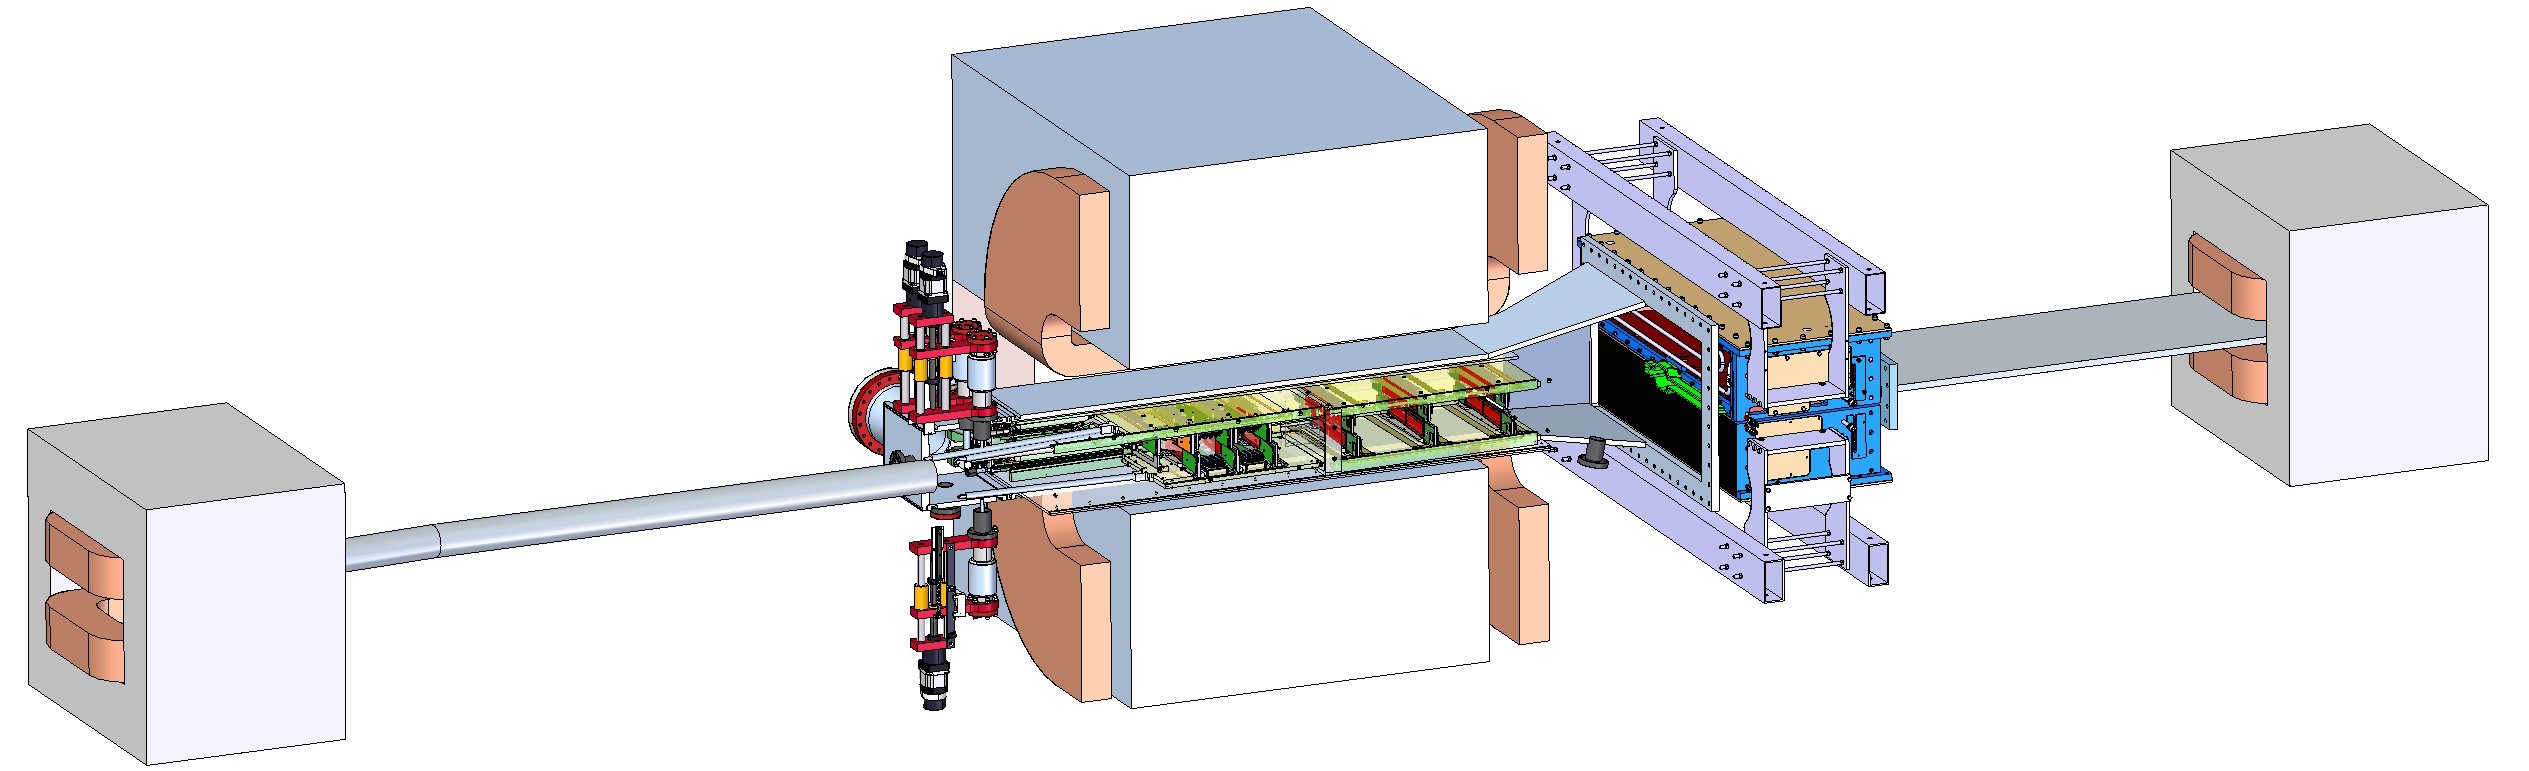
\includegraphics[width=\textwidth]{detector/figs/HPS-pic}
    \caption{View of the HPS setup.
    The beam direction is left to right.}
    \label{fig:hps-pic}
\end{figure}

\section{Beamline}
\label{sec:beamline}

HPS uses the CEBAF (Continuous Electron Beam Accelerator Facility) accelerator at Jefferson Lab (Figure \ref{fig:cebaf}).
CEBAF is a recirculating linac, where the electron beam can take multiple passes through the same set of accelerating cavities.
%CEBAF has a continuous duty cycle because it uses superconducting accelerating cavities, which can be operated continuously without 
The superconducting RF cavities used at CEBAF allow a continuous duty cycle, where beam bunches pass through the accelerator at 1500 MHz without interruption.
A system of RF separators delivers beam to each of four experimental halls at 250 or 500 MHz, and allows each hall to select its own beam energy.
HPS is installed in Hall B, the hall that typically operates at the lowest beam current.

The main detector in Hall B is CLAS (CEBAF Large-Acceptance Spectrometer), which is used for precision nuclear physics experiments with low-current (sub-$\mu$A) beams of electrons or photons. CEBAF recently underwent a major upgrade to increase the maximum beam energy from 6 GeV to 12 GeV, and add a new experimental hall (Hall D).
CLAS is undergoing a major rebuild (to become the CLAS12 detector) for 12 GeV operation, and this work is still in progress.
The 2015 and 2016 HPS runs were conducted after CEBAF began 12 GeV operations but before much of CLAS12 was complete; HPS is the first Hall B experiment of the 12 GeV era, albeit not operating at 12 GeV (the maximum field of the HPS magnets limits HPS to 6.6 GeV beam).

The injector energy is 100 MeV and one pass through the linacs adds 2.2 GeV to the beam energy, so in normal operation, the available beam energies at Hall B are 100 MeV + $n*2.2$ GeV where $n$ is 1 through 5.
During the 2015 engineering run, a mechanical problem disabled one of the two CEBAF helium liquifiers.
With half the cooling power, the superconducting cavities could only be run at half the nominal gradient.
HPS took the opportunity to run at 1.056 GeV, an energy that is not normally available.

HPS relies on the continuous beam structure at CEBAF to reduce pileup.
A beam bunch arrives at HPS every 2 ns, which is comparable to the time resolution of the detectors.
This means that beam backgrounds are spread in time as uniformly as possible.
A larger bunch spacing or lower duty cycle would increase the amount of beam background that overlaps an event of interest.

\begin{figure}[htp]
    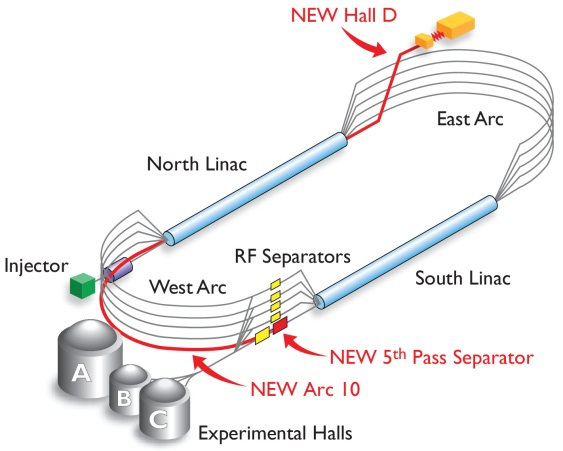
\includegraphics[width=0.6\textwidth]{detector/figs/cebaf}
    \caption{Schematic of the CEBAF accelerator, highlighting components added for the 12 GeV upgrade.}
    \label{fig:cebaf}
\end{figure}

\subsection{Hall B Beamline and Instrumentation}
\label{sec:beamline_hallb}

\begin{figure}[htp]
    \begin{center}
        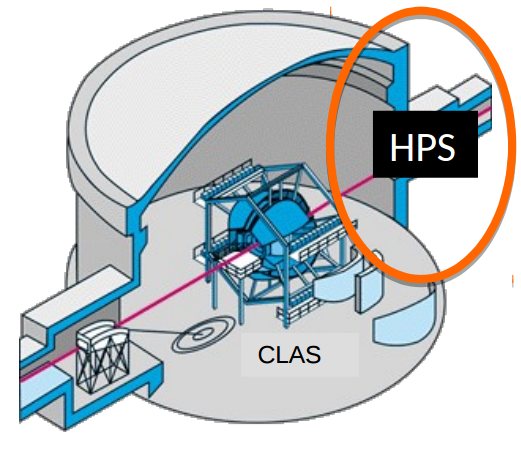
\includegraphics[width=0.5\textwidth]{detector/figs/hallb}
    \end{center}
    \caption{Location of the HPS setup, in the downstream alcove of Hall B.
    The beam direction is left to right.}
    \label{fig:hallb}
\end{figure}

HPS is installed in the downstream alcove of Hall B: see Figure \ref{fig:hallb}.
Since CLAS12 construction is in progress, a plain beam pipe was installed to pass the beam through CLAS, and HPS operations were limited to nights and weekends to allow CLAS construction to continue.

The Hall B beamline can be configured for delivery of both electron and photon beams.
Soon after it enters the hall, the CEBAF electron beam passes through a large ``tagger'' magnet.
If a target is positioned upstream of the tagger magnet, a beam of bremsstrahlung photons can be sent to experiments while the tagger magnet sends the beam to a dump (the ``tagger dump'') and the bremsstrahlung electrons to wire chambers (``tagging'' the energy of each photon).
For HPS operation the beamline is run in the electron configuration (tagger magnet de-energized, electrons to HPS and main dump), but the photon configuration (tagger magnet energized, electrons to tagger dump) is still used for beam setup since it allows for tuning the upstream part of the beamline without impacting the beam at HPS.

The Hall B beam instrumentation consists of beam position monitors (BPMs), halo monitors, wire scanners, viewers, and a Faraday cup.

BPMs detect the current induced by passing beam bunches in order to measure the current and/or position of the beam.
Since this is a noncontact measurement, BPMs operate continuously during operations and provide a record of beam changes during data taking.

Halo monitors are small particle detectors (mostly scintillation counters) positioned around the beam pipe.
If the beam is obstructed, defocused or missteered, it will scatter into the halo monitors.
%The halo monitors can be used as part of the fast shut down (FSD) system.

Wire scanners consist of a set of wires mounted on a motorized frame.
The beam position and size is measured by scanning the wires across the beam; the halo counter rates increase in proportion to the amount of beam subtended by a wire.
An example wire scan is shown in Figure \ref{fig:beamsize}.
All harps have at least one vertical and one horizontal wire; some have a diagonal ($45^\circ$) wire for measuring the beam tilt and/or thicker wires for measuring the tails of the beam.

\begin{figure}[htp]
    \begin{center}
        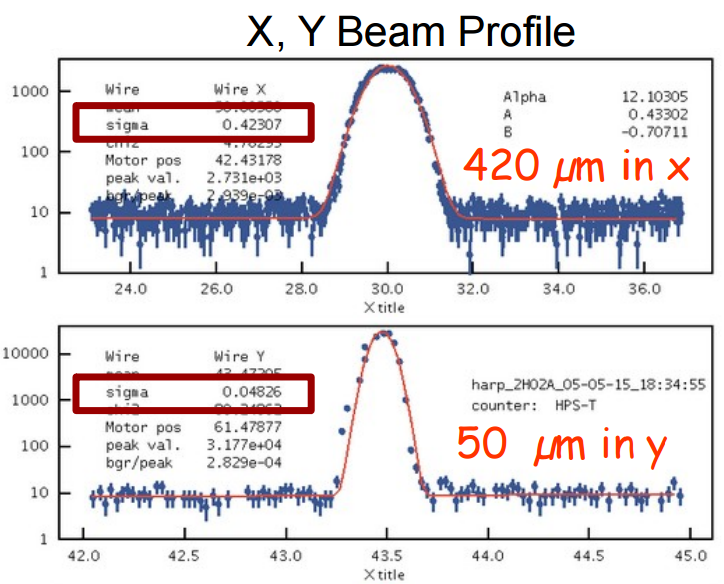
\includegraphics[width=0.5\textwidth]{detector/figs/beamsize}
    \end{center}
    \caption{A representative wire scan measurement of the beam size.
        This scan was taken using the 2H02 wire scanner just upstream of HPS, and reflects the beam size seen at the HPS target.
    This wire scan was taken early in the 2015 run; the beam size in X was reduced later in the run, and all physics data was recorded with a beam size of roughly $150\times 50$ $\mu$m.
    }
    \label{fig:beamsize}
\end{figure}

Beam viewers consist of a thin screen that emits light when the beam passes through it, and a video camera for viewing the shape and position of the beam.
Fluorescent screens are sensitive but are susceptible to saturation and blooming effects, and are most useful for viewing the beam position.
A screen using optical transition radiation (OTR) is dimmer, but does not saturate and accurately shows the beam shape.
One fluorescent screen is mounted in front of the Hall B tagger dump.
Two fluorescent screens of different types, and one OTR screen, are mounted on a motorized carousel in front of the Hall B main dump.

The Hall B beamline terminates in a Faraday cup, which directly measures the beam charge.
This is the most accurate measurement of the beam current.

\subsection{Beam Quality and Protection}
\label{sec:beam_quality}
HPS has two primary concerns regarding the beam.
First, since the SVT is so close to the beam, the SVT must be protected both from beam being directed into the silicon and causing damage, and from stray beam electrons hitting the inner regions of the active silicon and adding to the detector pileup.
This implies strong beam protection controls and low beam halo.
Second, a small beam spot is important for event quality cuts; if the beam spot is small (ideally, smaller than detector resolution), poorly reconstructed tracks or vertices that are not consistent with an origin at the beam spot can be rejected.
%Beyond a small beam spot, this implies a stable beam, since beam motion will smear the effective beam spot size, and a repeatable beam position from run to run.

Active beam protection is provided by the CEBAF fast shutdown (FSD) system.
The FSD system is an interlock which, when triggered, shuts off the electron gun in the injector.
In addition to the large amount of beam instrumentation that is normally connected to the FSD, the set of halo counters closest to HPS were used to provide an FSD signal.
This halo counter FSD was configured so that an abnormally high rate on the halo counters (the threshold being set as low as possible without causing spurious beam trips) would trip the beam in 1 ms.
If the beam were to move into the SVT sensors, it would hit the inactive edge of the silicon (0.5 mm from the nominal beam position) first.
The beam scattering from the silicon would trip the halo counter FSD, hopefully before the beam could reach the active silicon (1.5 mm from the nominal beam position).

A collimator provides passive beam protection.
The collimator is a tungsten plate 1 cm thick with machined slots of different widths, mounted on a linear shift so the appropriate slot can be selected and positioned precisely.
For the 2015 run, the 3 mm slot was used; this slot width is equal to the gap between the active regions of the SVT.
If the beam were to move into active silicon, the collimator would absorb and spread the beam enough that the silicon would not be damaged in the time it would take for the FSD to stop the beam.
%beam protection, FSD

Measurements of the beam halo, such as shown in Figure \ref{fig:beam-tails}, show that the beam profile does not deviate from a Gaussian for five orders of magnitude; the rate of beam electrons outside of $\pm 0.5$ mm is $10^{-5}$ of the beam current.
At this level, the rate of beam halo electrons hitting the innermost strips of the SVT is less than the rate of scattered electrons from the target.

\begin{figure}[htp]
    \begin{center}
        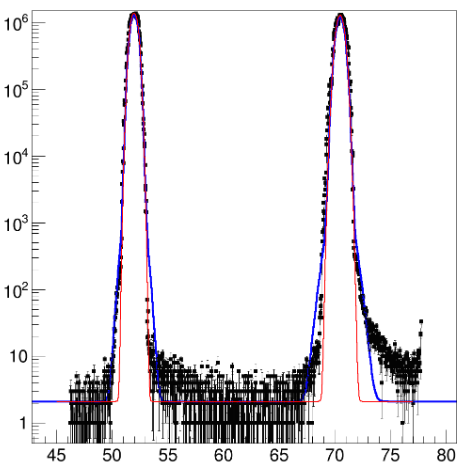
\includegraphics[width=0.5\textwidth]{detector/figs/beam-tails}
    \end{center}
    \caption{A wire scan measurement of the beam halo.
    The black data points show the halo counter rates as a function of motor position.
    The two peaks correspond to the horizontal and vertical wires (each wire is iron, 1 mm diameter) crossing the beam.
    The red curve is a fit to the Gaussian core of the beam, and the blue curve is its convolution with the wire size.
    The data is consistent with the fits over five orders of magnitude, indicating that the beam halo is of that level.
    }
    \label{fig:beam-tails}
\end{figure}

HPS originally requested a beam size that was smaller in Y than in X.
Since the vertex resolution is better in Y ($\sim 150$ $\mu$m) than in X ($\sim 300$ $\mu$m), and target heating was incorrectly believed to limit the minimum safe beam size, the desired beam shape was narrow ($\sim 50$ $\mu$m) in Y and wider ($\sim 300$ $\mu$m) in X.
One challenge in making such an asymmetric beamspot is that the beam tilt must be precisely controlled.
As shown in Figure \ref{fig:beamsize}, this was achieved.
It was later realized that target heating was not a serious concern, and all 2015 physics data was recorded with a beam size of $\sim 50$ $\mu$m in Y and $\sim 150$ $\mu$m in X.

\subsection{HPS Beamline Elements}

The HPS chicane, shown in Figure \ref{fig:hps-pic}, consists of three dipoles with fields in the vertical direction.
The three magnets of the chicane are repurposed from a past Hall B experiment.
The detector is installed in the central magnet (the ``pair spectrometer'' magnet), which is a 18D36 magnet (pole length 91.44 cm, width 45.72 cm), and was operated at a field strength of 0.24 T for the 2015 run.
The outer magnets are identical ``Frascati''-type magnets, equidistant from the analyzing magnet and operated at equal field strengths, such that the $\int B dl$ of each Frascati magnet is half that of the analyzing magnet (and opposite in sign).
This ensures that the beam trajectory downstream of the chicane is the same whether or not the chicane is energized.

A series of connected vacuum chambers constitute the HPS beam path.
A short rectangular chamber upstream of the pair spectrometer magnet provides feedthroughs for SVT services (motion, cooling, power, data), further described in Section \ref{sec:svt_services}.
A long rectangular chamber (inherited with the pair spectrometer magnet) fills the magnet bore and extends downstream; the downstream segment flares outward to allow charged particles to bend.
The next chamber (shown in Figure \ref{fig:ecal_chamber}) closes off the vacuum chamber, except for a slot-shaped channel that allows the beam and the sheet of flame to pass through to the dump; the ECal (which does not operate in vacuum) closely surrounds the slot on top and bottom.

\begin{figure}[htp]
    \begin{center}
        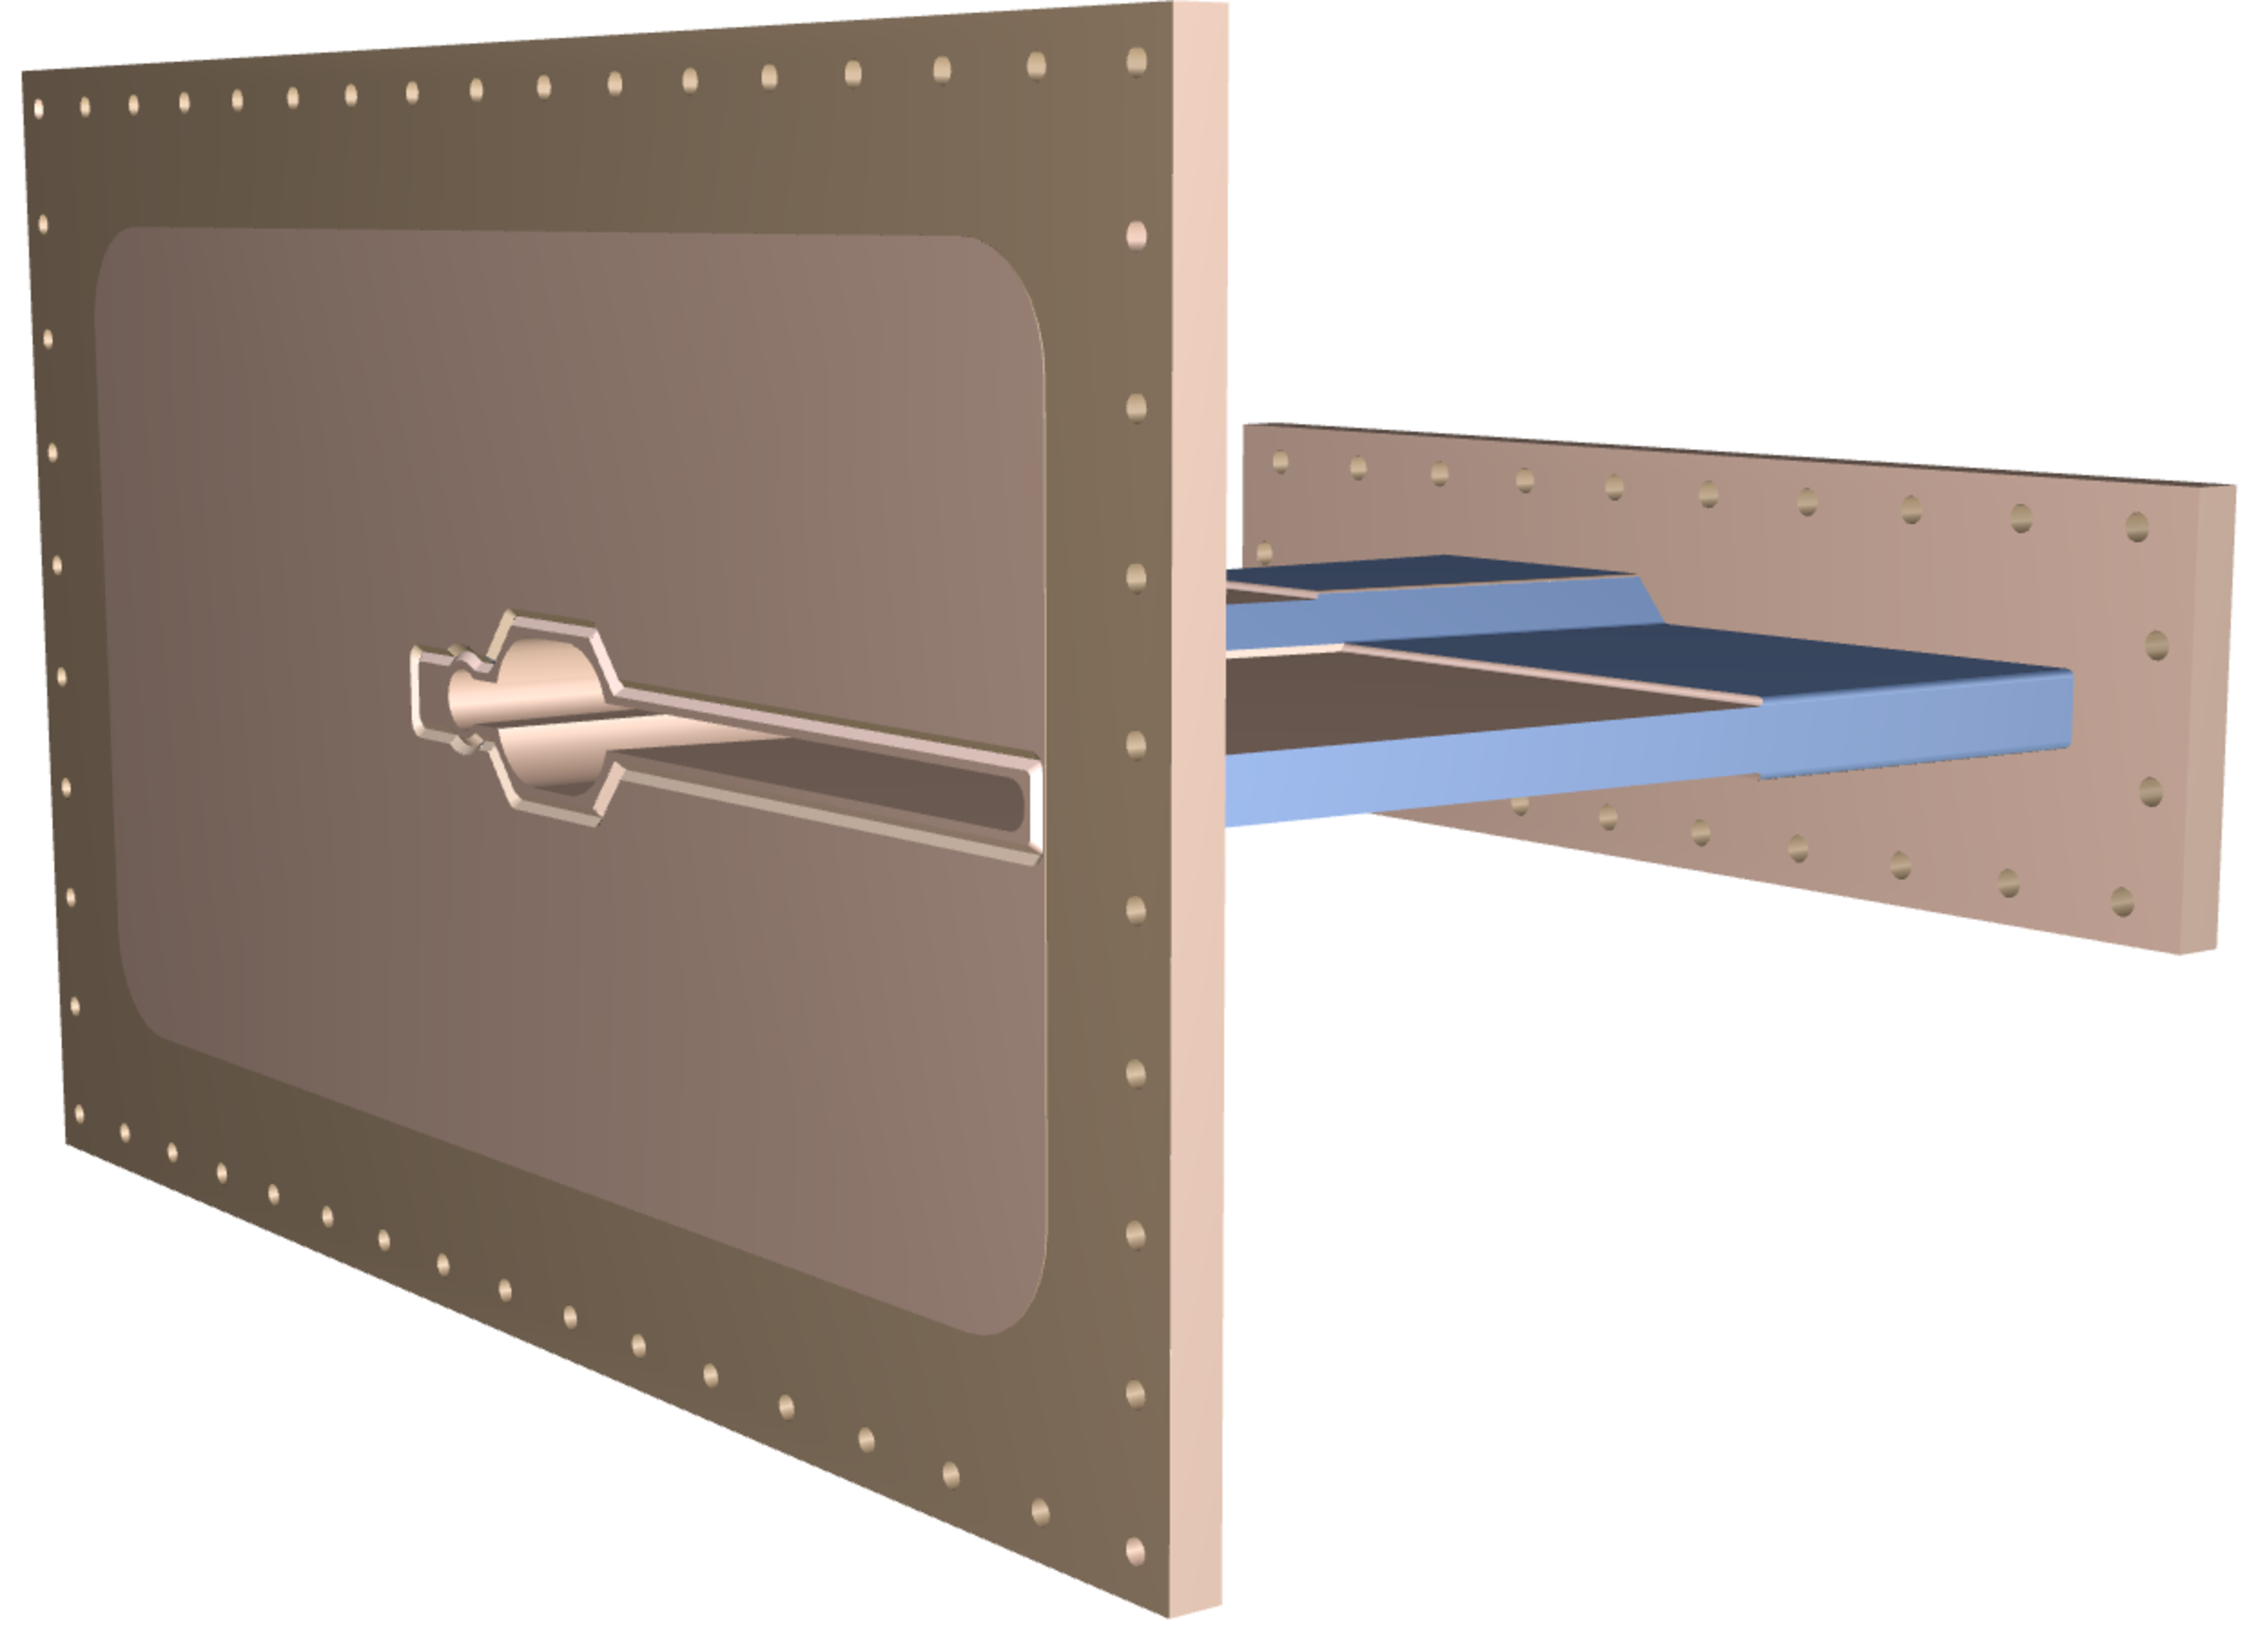
\includegraphics[width=0.5\textwidth]{detector/figs/ecal_vac}
    \end{center}
    \caption{A rendering of the ECal vacuum chamber.
    The large rectangular flange closes off the pair spectrometer vacuum chamber.
    The slot has a complex shape to pass different types of particles radiating from the target.
    From left to right: the round tube passes bremsstrahlung photons, the oval tube passes the beam (which is enlarged by small-angle scattering) and M{\o}ller-scattered electrons, and the wide slot passes bremsstrahlung electrons.
    The walls of the slot are quite thin and a strut of aluminum honeycomb (not visible) supports it against air pressure.
    }
    \label{fig:ecal_chamber}
\end{figure}

The HPS target is a set of foils mounted on a common frame.
There are two tungsten foils, one graphite foil, and one polyethylene foil.
The tungsten foils have design thicknesses of 0.125\% and 0.25\% radiation lengths; from measurements made during target assembly, the true thicknesses are 0.116\% and 0.223\%.
The 0.125\% $X_0$ foil is for runs at 1.1 and 2.2 GeV, and the 0.25\% $X_0$ foil is for runs at 4.4 and 6.6 GeV.
A linear shift moves the frame up and down so the foils can be moved in and out of the beam; since the target needs to be at the face of the magnet, and the linear shift is on one of the flanges of the upstream vacuum chamber, the target frame is cantilevered on a ceramic support rod.

\begin{figure}[htp]
    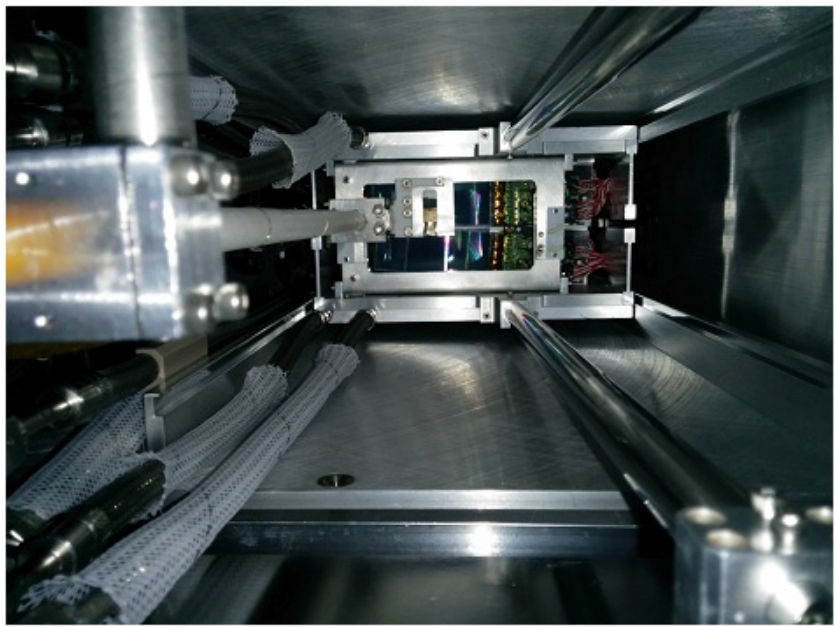
\includegraphics[width=\textwidth]{detector/figs/target_photo}
    \caption{Beam's-eye view of the HPS target and the front of the SVT after installation.
    The vertical rod from the target linear shift (foreground left), the ceramic support rod, and the target frame (center, offset to the right from the end of the support rod) are visible.
    }
    \label{fig:target_photo}
\end{figure}

\section{Silicon Vertex Tracker}

\begin{figure}[htp]
    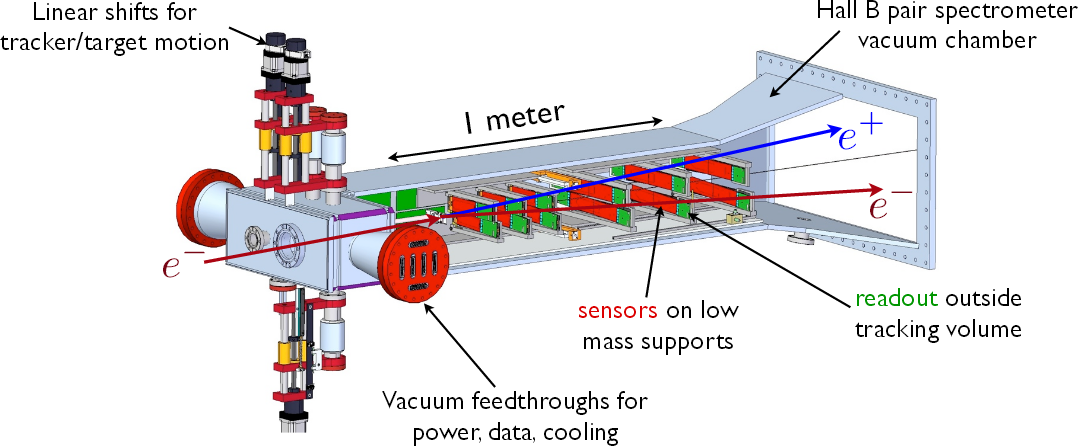
\includegraphics[width=\textwidth]{detector/figs/svt_cutaway}
    \caption{Schematic of the SVT and its support systems.}
    \label{fig:svt-schematic}
\end{figure}

\begin{figure}[htp]
    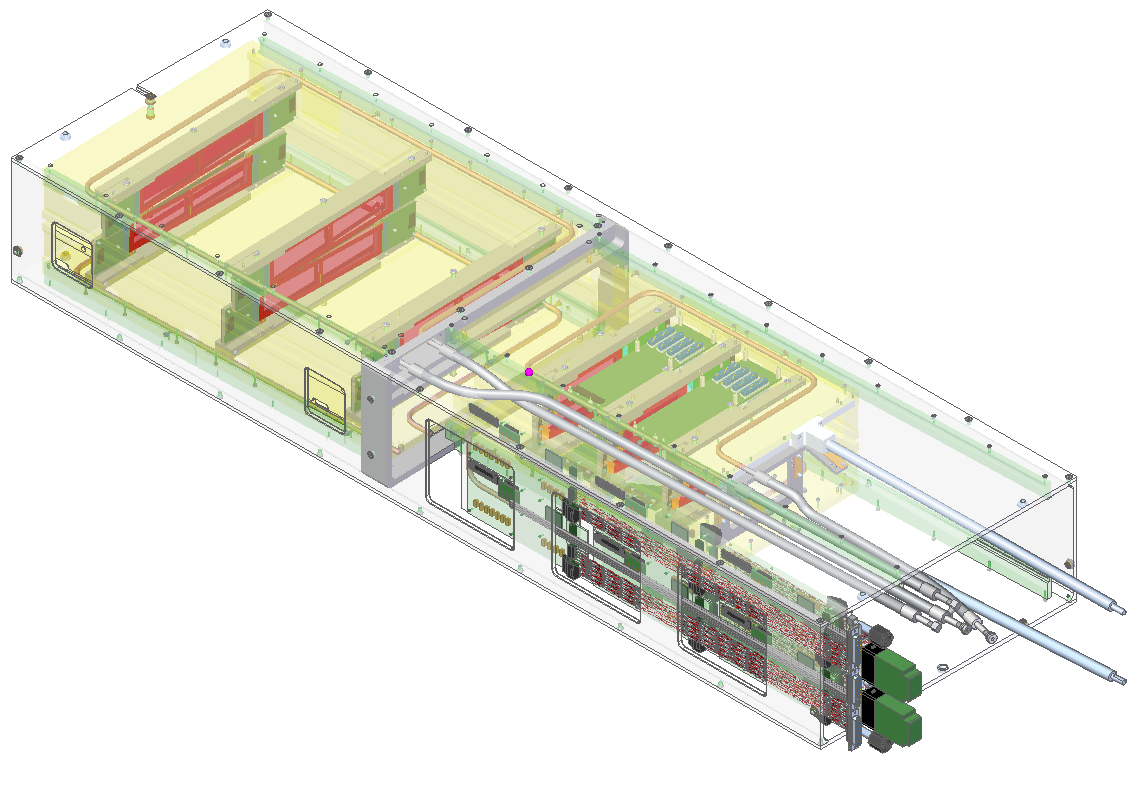
\includegraphics[width=\textwidth]{detector/figs/svt_drawing}
    \caption{Rendering of the SVT as built, showing cooling lines and motion levers.}
    \label{fig:svt-drawing}
\end{figure}

The silicon vertex tracker (SVT) measures track momentum and vertex position.

HPS uses silicon microstrips because they provide good time resolution, low mass, and high rate.
Because a microstrip sensor can only make a 1-D measurement (it identifies the strip that was hit, but not the hit position along the strip), each measurement station (called a ``layer'') uses two sensors at an angle relative to each other.
For HPS this stereo angle is kept small, so all sensors have their strips pointing roughly in the bend direction.
A small stereo angle is a compromise: it sacrifices measurement resolution in the strip direction, but it is less likely that two particles will create ``ghost hits'' when the strips they hit intersect each other.
The stereo angle is not uniform throughout the SVT (it is 100 milliradians in the upstream half, 50 milliradians in the downstream half), which prevents ghost hits from creating ghost tracks.

The SVT is made of six layers at different distances from the target: this number allows for 5-hit tracking even if a particle misses one layer.
Layer 1 is 10 cm from the target; this is the closest we can safely operate while allowing 500 $\mu$m distance from the beam to the edge of the sensors, which have a 1 mm border of inactive silicon.
Layer 6 is 90 cm from the target, just at the end of the uniform field region of the analyzing magnet; maximizing the length of the tracker maximizes the momentum resolution.
Layers 1--3 use single sensors; layers 4--6, where tracks have bent out to the sides, use two sensors joined end to end.
The layout of the six layers is summarized in Table \ref{tab:svt_layout}.

\begin{table}[htp]
    \begin{center}
        \caption{Layout of the HPS SVT.  The angle of stereo sensors is relative to the bend plane.}
        \begin{tabular}{lcccccc}   
            \hline \hline 
            Layer number & 1 & 2 & 3 & 4 & 5 & 6 \\      
            \hline
            nominal $z$, from target (cm)  & 10 & 20 & 30 & 50 & 70  & 90 \\ 
            Stereo Angle (mrad)  & 100 & 100 & 100 & 50 & 50 & 50 \\ 
            Bend-plane resolution ($\mu m$)  & $\approx$60 & $\approx$60 & $\approx$60 & $\approx$120 & $\approx$120 & $\approx$120 \\ 
            Non-bend resolution ($\mu m$)  & $\approx$6 & $\approx$6 & $\approx$6 & $\approx$6 & $\approx$6  & $\approx$6 \\ 
            Number of sensors  & 4 & 4 & 4 & 8 & 8 & 8 \\ 
            Nominal dead zone in $y$ (mm)  & $\pm1.5$  & $\pm3.0$  & $\pm4.5$  & $\pm7.5$  & $\pm10.5$ & $\pm13.5$  \\ 
            Module power consumption (W) & 6.9 & 6.9 & 6.9 & 13.8 & 13.8 & 13.8 \\
            \hline \hline
        \end{tabular}
        \label{tab:svt_layout} 
    \end{center}
\end{table}

Because the SVT operates in a high magnetic field and in vacuum, materials must be compatible.
All materials are checked for vacuum compatibility by pumping test samples to high vacuum in a test chamber.
Only nonmagnetic materials are used; inductors used on the frontend boards are air-core (instead of ferrite, which would saturate).

\subsection{Sensors and Readout}
HPS uses silicon microstrip sensors that were originally produced for the run IIb upgrade of the D{\O} detector at Fermilab.
This upgrade would have replaced the entire SMT (silicon microstrip tracker).
The full SMT upgrade was cancelled in favor of an insertable Layer 0, but not before sensors had already been procured.
The sensors used for HPS are those that would have been used for layers 2--5 of the new D{\O} tracker.

The HPS sensors are single-sided p+n with AC-coupled readout: the bulk is lightly doped n-type silicon with $<$100$>$ crystal orientation, and the strip implants are strongly p-type doped.
The strips are biased through polysilicon resistors at the ends of the strips, and capacitively coupled to aluminum readout strips that run on top of the strips.
Only every other strip is read out; the ``readout'' strips capacitively couple to the intermediate ``sense'' strips, so a hit in a sense strip splits its charge between the neighboring readout strips.

Radiation damage limits the useful lifetime of silicon sensors.
Incident particles can displace silicon atoms from their places in the crystal lattice, which effectively converts the n-type bulk of the sensor to p-type (type inversion).
This increases the depletion voltage, so the sensor bias must be increased to keep the same charge collection efficiency; the sensor lifetime is therefore limited by the breakdown voltage of the sensor.
The defects also increase the leakage current, which leads to increased sensor heating.
The HPS sensors are specified to have a breakdown voltage of greater than 350 V, and a further selection was made to only use sensors with a breakdown voltage in excess of 1000 V.

\begin{table}[htp]
    \begin{center}
        \caption{Specifications of the SVT sensors.
        Breakdown voltage specification is value accepted for use in HPS; procurement specification was looser.}
        \begin{tabular}{lc}   
            \hline \hline
            Thickness & 320 $\mu$m \\
            Overall area (L$\times$W) & 100 mm $\times$ 40.34 mm\\
            Active area (L$\times$W) & 98.33 mm $\times$ 38.34 mm\\
            Strip pitch (count) & 30 $\mu$m (1277)\\
            Readout pitch (count) & 60 $\mu$m (639)\\
            Depletion voltage & 110-130 V (typical)\\
            Breakdown voltage & $>$1000 V\\
            \hline \hline
        \end{tabular}
        \label{tab:sensor_spec} 
    \end{center}
\end{table}

The sensors are read out by the APV25 readout chip \cite{french_design_2001}.
This chip was developed for silicon microstrip readout in the CMS tracker.
Because the APV25 can read out multiple consecutive samples of its shaper waveform, it can be used for pileup rejection and high-precision hit time reconstruction.
This is an essential feature for HPS and other experiments (notably the Belle II SVD \cite{liu_belle_2012}) with CW beam and high pileup.

Each APV25 chip has 128 input channels.
One channel consists of a charge-sensitive preamp with an optional inverter, CR-RC shaper, and 192-cell analog pipeline.
We run the chip with a 24 ns clock: the design clock period is 25 ns to match the LHC bunch crossing period, but 24 ns is an even multiple of the standard JLab clock.
On each clock, each channel samples its shaper output and stores it in a cell of its pipeline.
On a trigger, each channel reads out the appropriate pipeline cell, and the chip multiplexes the 128 signals onto a single differential current output.
A configurable ``latency'' setting determines which pipeline cells are read out; since the cells of interest are those that were written at the time of the triggering event, the latency should approximately equal the trigger delay.

\begin{figure}[htp]
    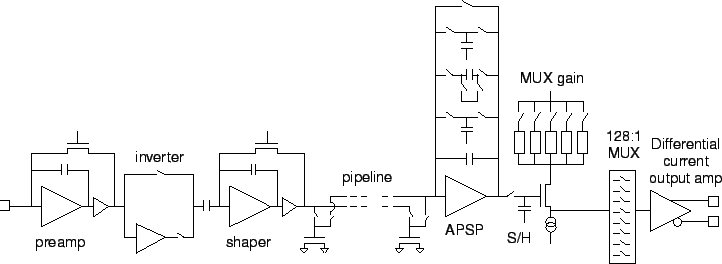
\includegraphics[width=\textwidth]{detector/figs/apv25}
    \caption{Schematic of the APV25. The APSP (analog pulse shape processor) is disabled in the ``multi-peak'' readout mode used by HPS.}
    \label{fig:apv25}
\end{figure}

HPS runs the APV25 in its ``multi-peak'' readout mode, which allows us to read out six consecutive pipeline cells for each trigger.
Six samples per trigger, combined with knowledge of the shaper pulse shape (from an offline calibration), allows us to fit the shaper output to the sum of one or two pulses.
The result is a reconstructed hit time and amplitude that is unaffected by a pileup hit that comes before or after the hit of interest.

\subsection{Mechanical Support}
\label{sec:svt_mechanical}

The base unit of the SVT is a ``half-module'' comprising a low-mass support structure, sensors, and hybrid readout circuit boards.
Half-modules are the only unit of the SVT that cannot be disassembled and reworked.
Two types of half-modules are used: layers 1--3 use single-ended half-modules with one sensor and hybrid each, and layers 4--6 use double-ended half-modules with two sensors and hybrids each.
A single half-module provides a single measurement (axial or stereo) for one half (top or bottom) of a layer.

\begin{figure}[htp]
    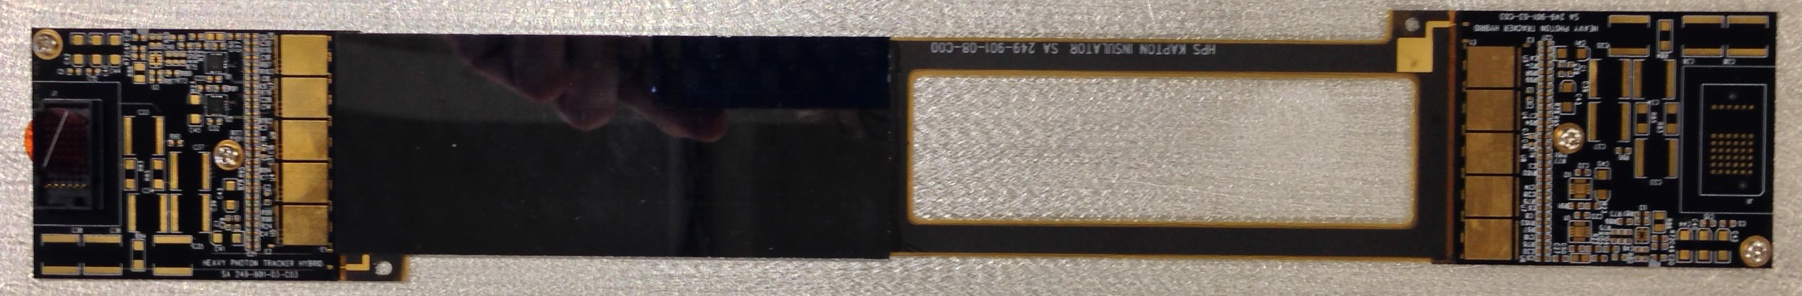
\includegraphics[width=\textwidth]{detector/figs/l456_hm}
    \caption{One half-module for L4--6. The two hybrids (without readout chips, which would be mounted on the gold pads) are at the left and right ends. One sensor is in place, on the left. The carbon fiber support and Kapton passivation layer are visible on the right.}
    \label{fig:l456_hm}
\end{figure}

The hybrid circuit board carries the APV25 readout chips, and connects the sensor to the rest of the DAQ.
The input channels of the APV25 chips are wirebonded directly to the sensor; the APV25 power, output channels, and control lines are wirebonded to the hybrid.
The hybrid also carries filter capacitors for the sensor bias, and temperature sensors to monitor the sensor temperature.

The carbon fiber support structure provides structural support for the silicon, and acts as a ground plane for the half-module.
A layer of Kapton insulation isolates the carbon fiber from the back surface of the sensor, which is held at high voltage.
The carbon fiber and Kapton are thinner than the silicon and contribute negligibly to the material seen by particles; cutouts further reduce any effect.
The sensors and hybrids are glued to the support structure with epoxy.

Two half-modules are paired back-to-back to form a ``module.''
The axial half-module is oriented with its strips pointing in the bend direction; the stereo half-module is rotated so it dips into the beam plane on the positron side (where beam backgrounds are less intense).
The modules are assembled using pairing fixtures, which are machined to set the edges of the sensors at precisely the correct height and angle.

\begin{figure}[htp]
    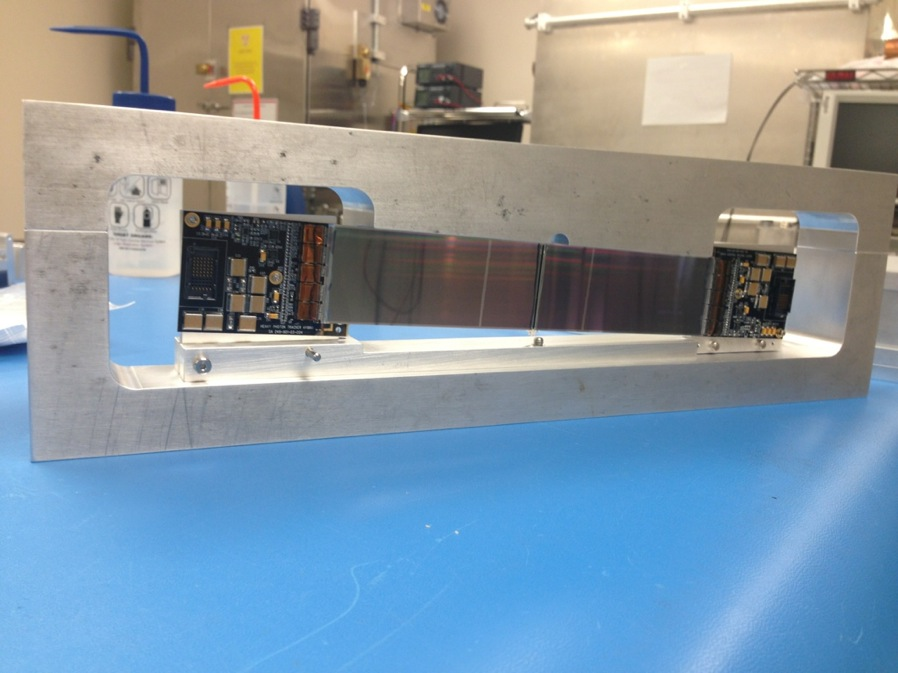
\includegraphics[width=\textwidth]{detector/figs/pairing_l456}
    \caption{The L4--6 pairing fixture, with one half-module in place.}
    \label{fig:l456_pairing}
\end{figure}

The aluminum module support holds the half-modules at both ends.
Heat generated by the hybrids is pulled out through the module support, which is in close thermal contact with the APV25 chips and the sensors through parallel paths so that the sensors can be kept colder than the APV25 chips.
The module support and the half-modules contract at different rates when the SVT is cooled to its operating temperature, so the module support must apply constant tension to keep the half-modules flat.
This is done with a spring pivot on one side of the module support.

\begin{figure}[htp]
    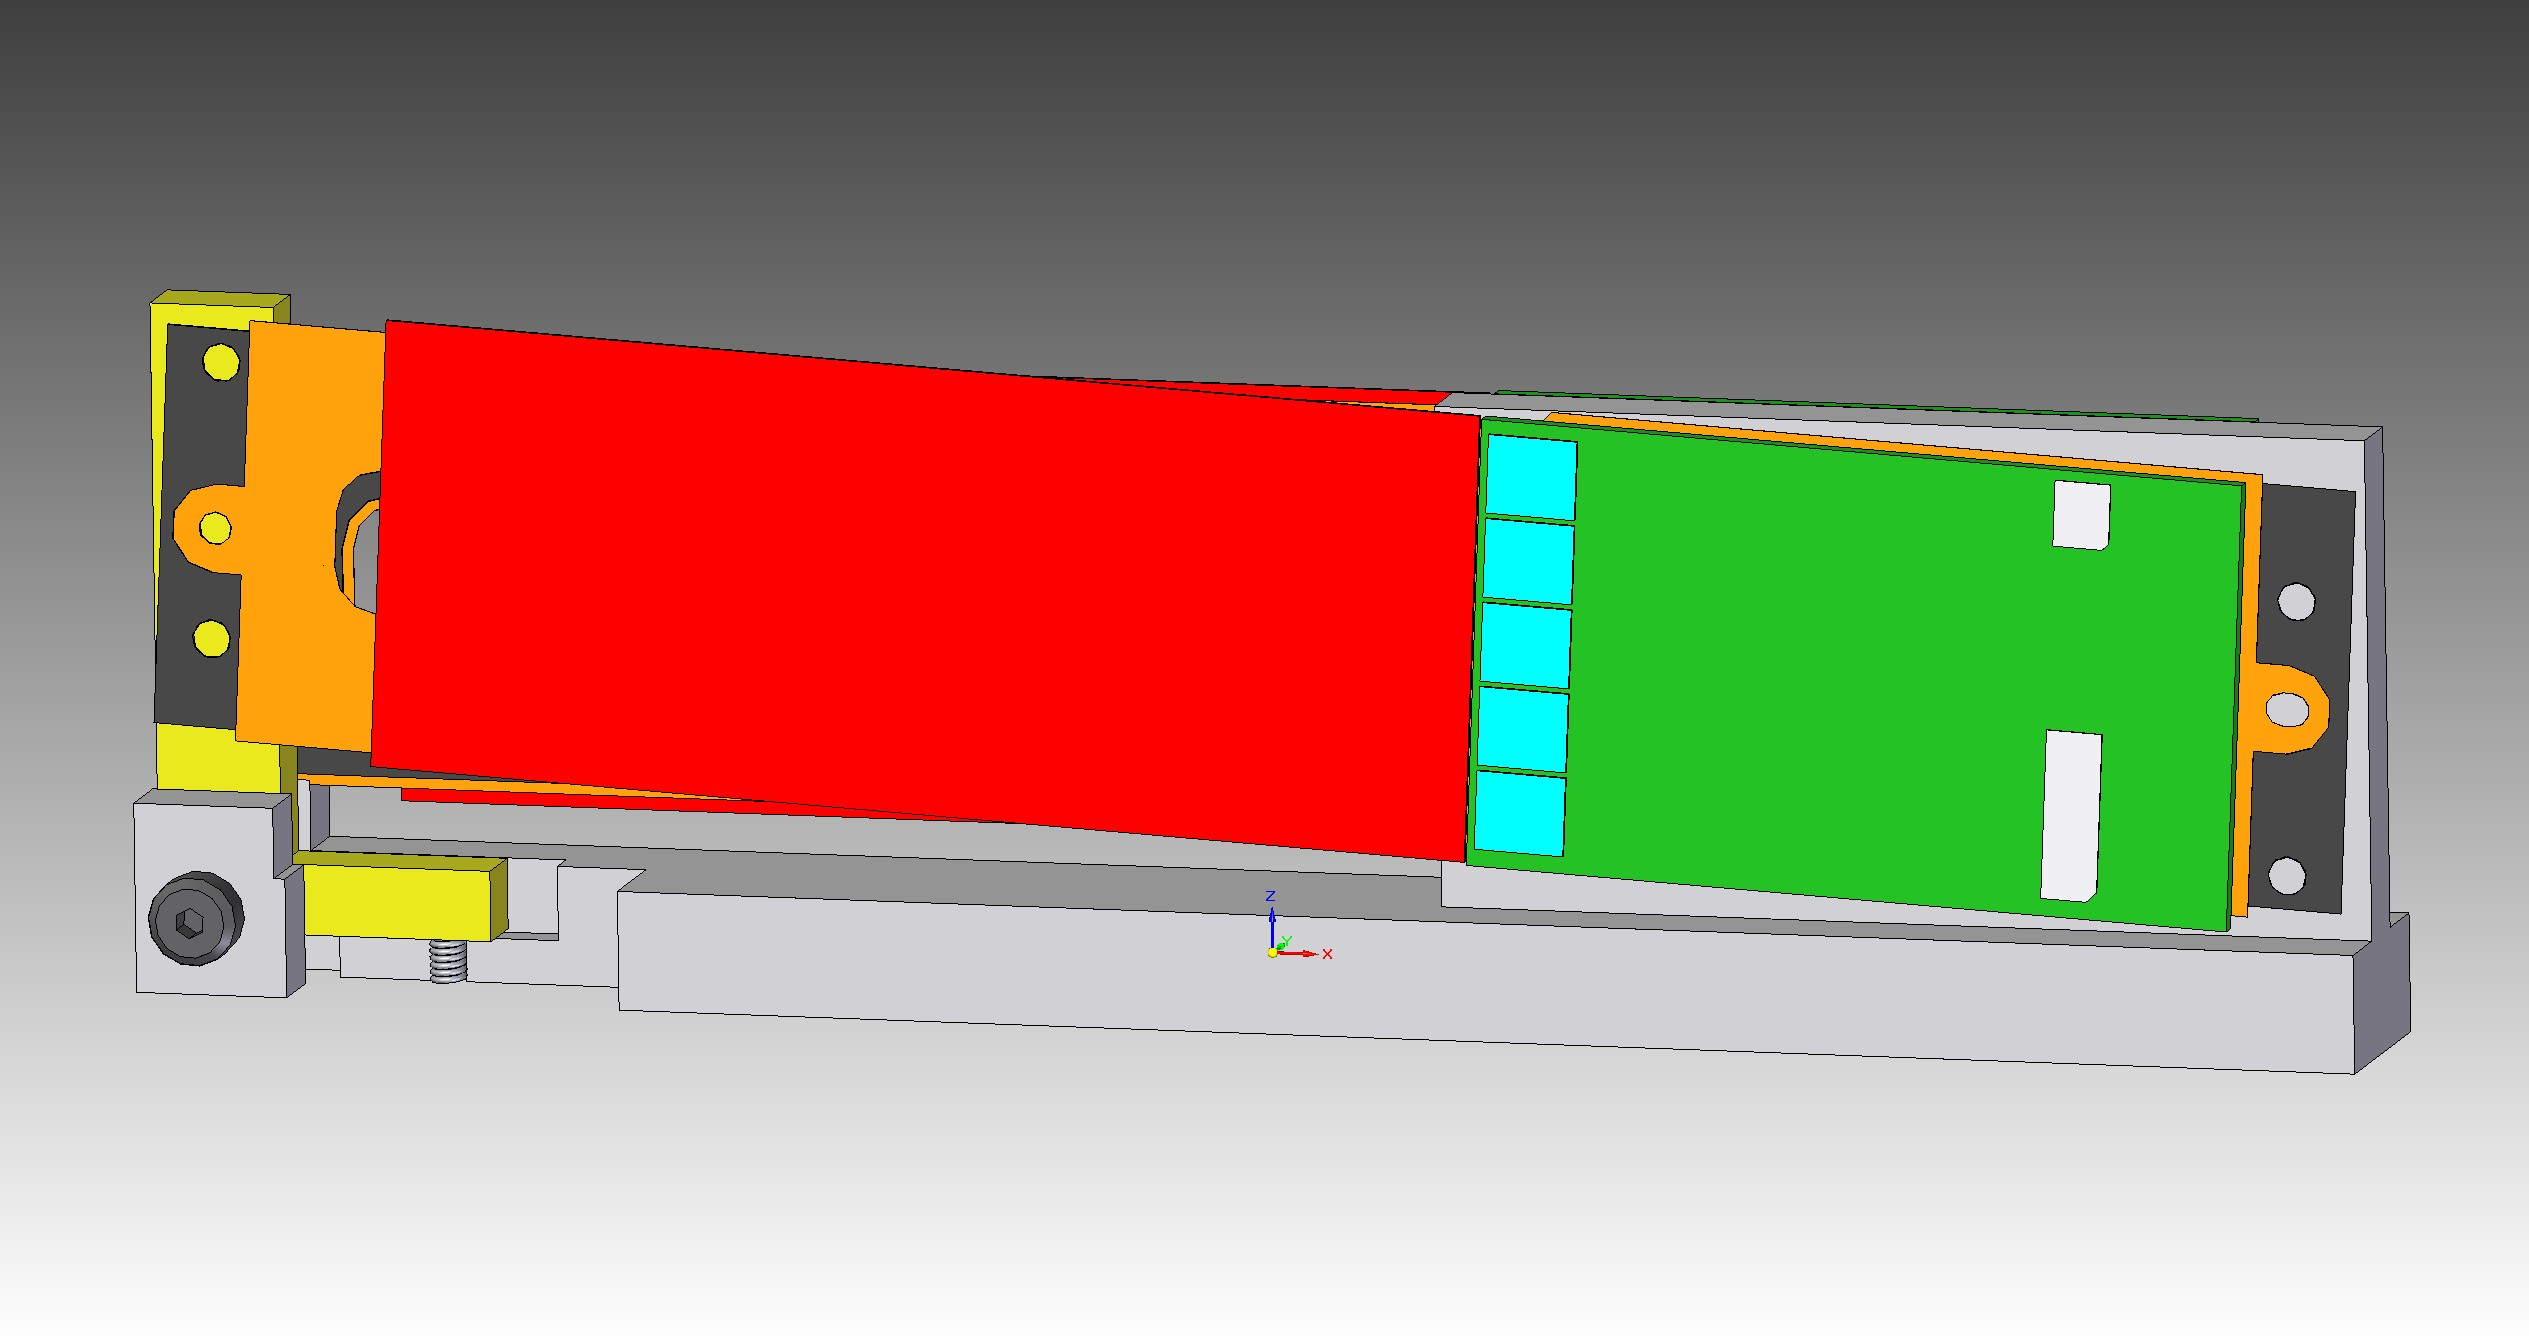
\includegraphics[width=0.5\textwidth]{detector/figs/svt_l123_drawing}
    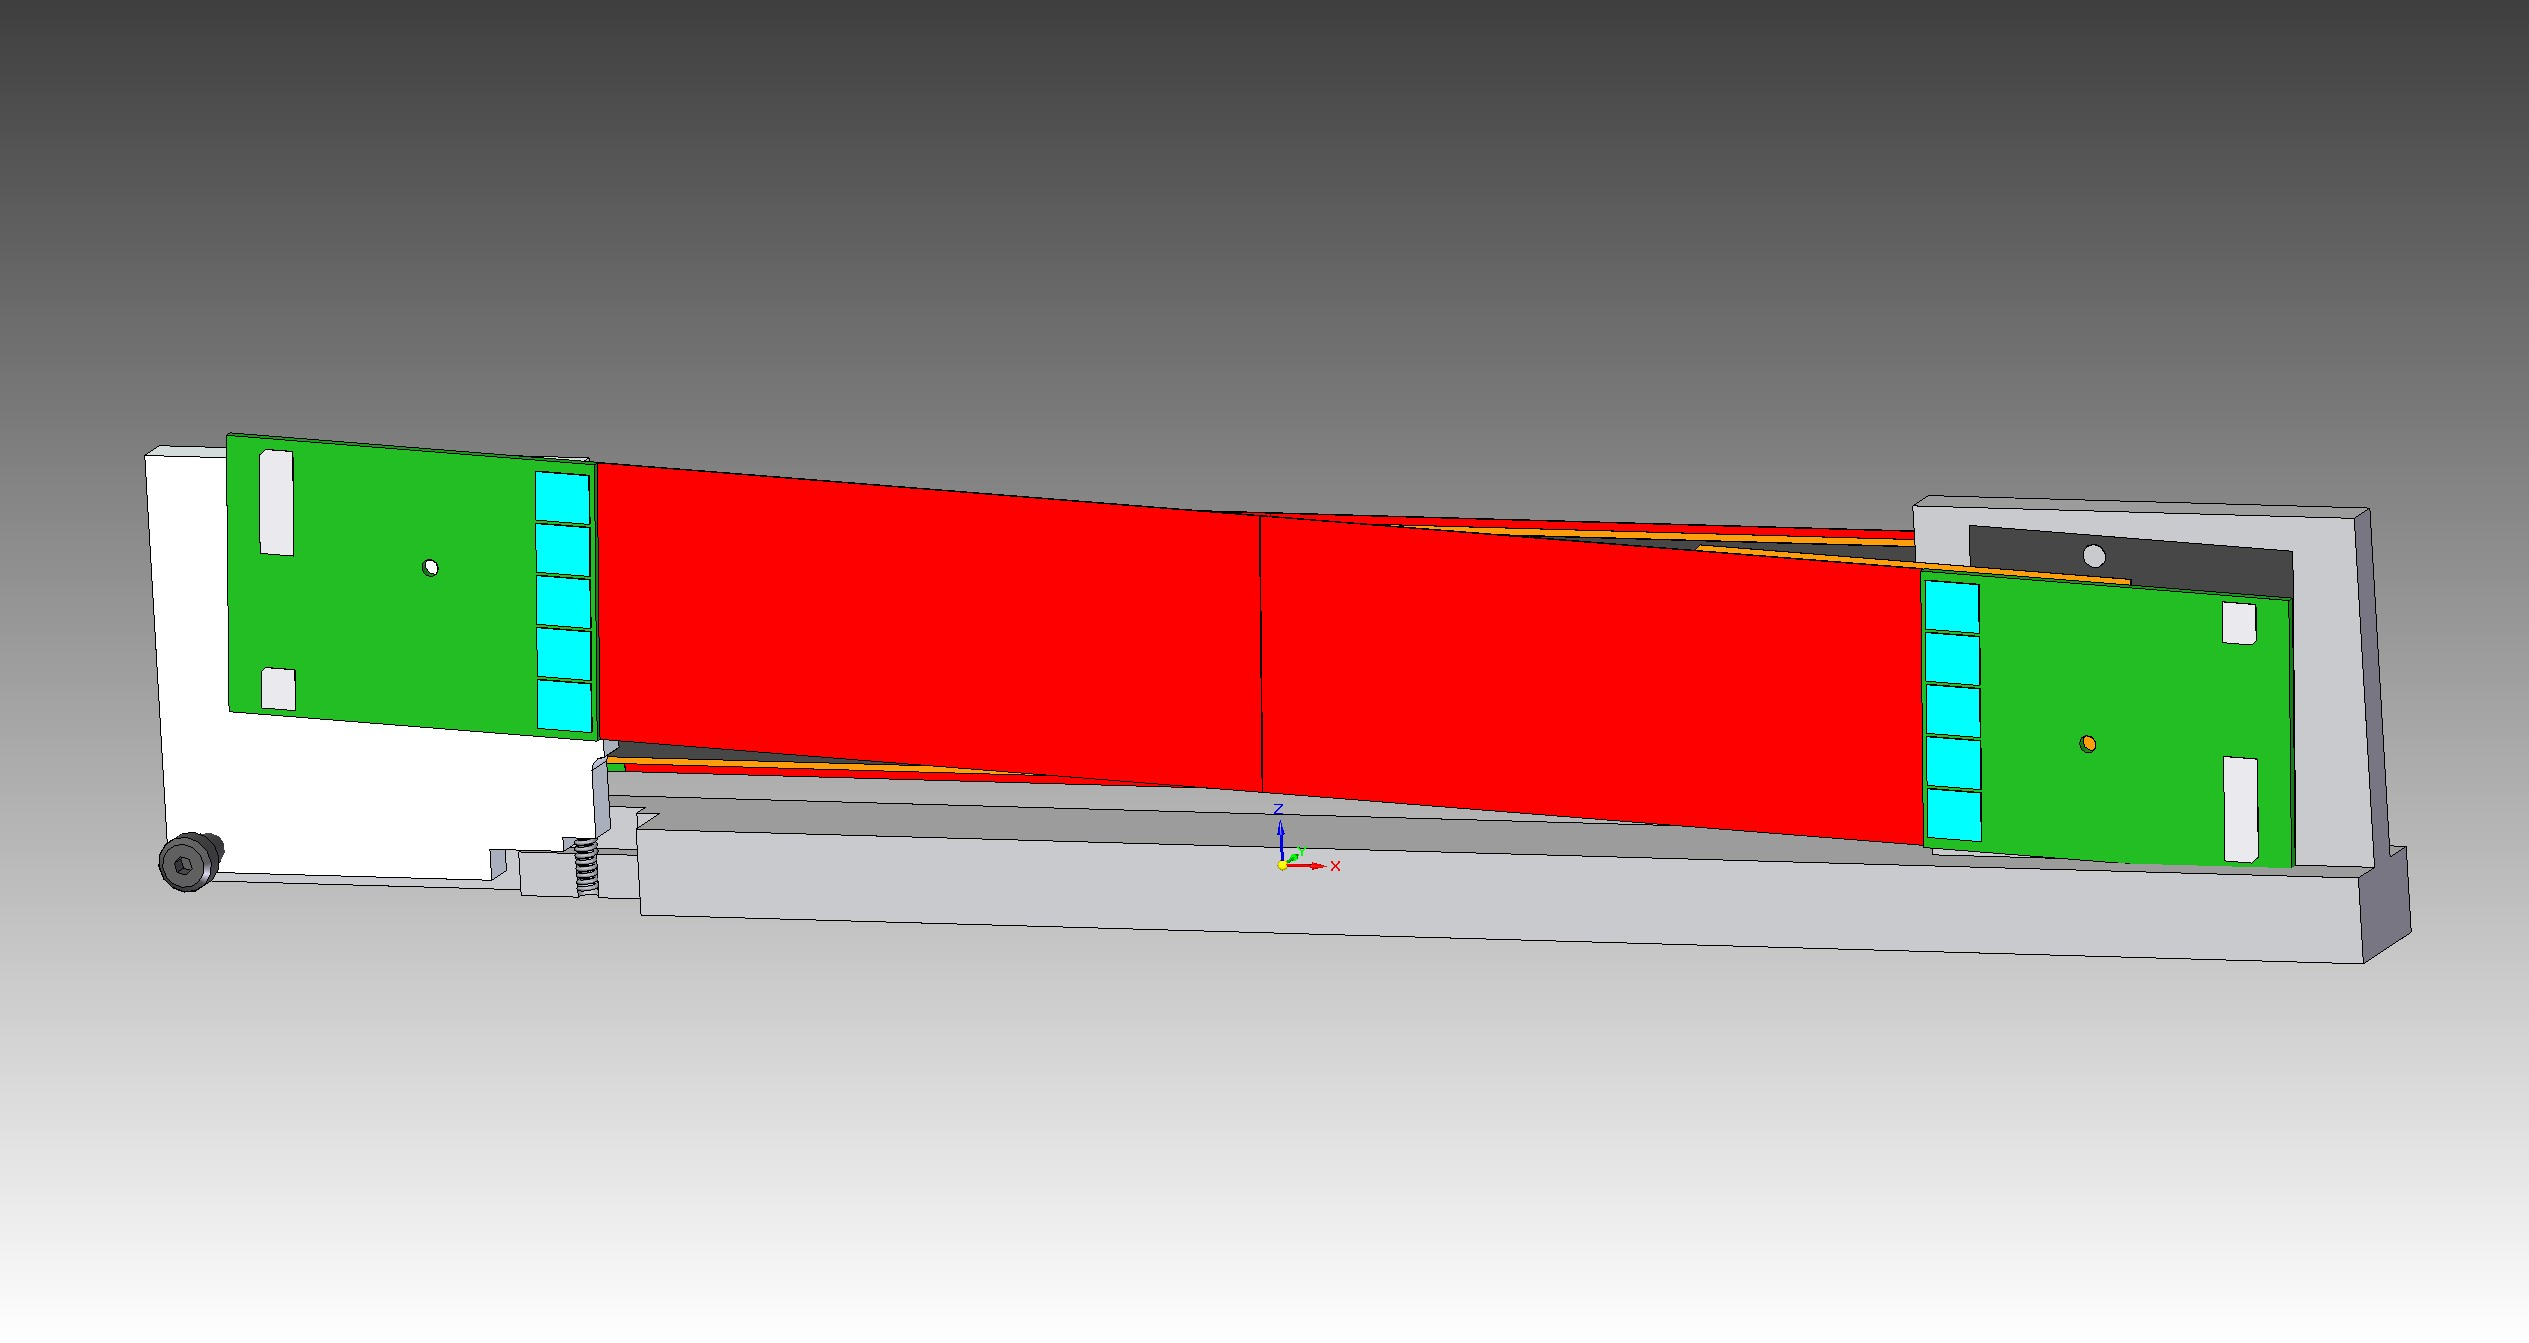
\includegraphics[width=0.5\textwidth]{detector/figs/svt_l456_drawing}
    \caption{Renderings of the L1--3 (left) and L4--6 (right) module designs, with cutaways to show the spring pivots that hold the silicon under constant tension.}
    \label{fig:svt-module-drawing}
\end{figure}

Three modules are mounted on a common aluminum support structure to form a ``U-channel.''
The sidewalls add to the rigidity of the U-channel and shield the sensors from thermal radiation.
The module mounting surfaces are recessed by the correct amounts to put the layers at the correct distances from the beam.
The SVT is divided into four U-channels: top and bottom L1--3, top and bottom L4--6.

\begin{figure}[htp]
    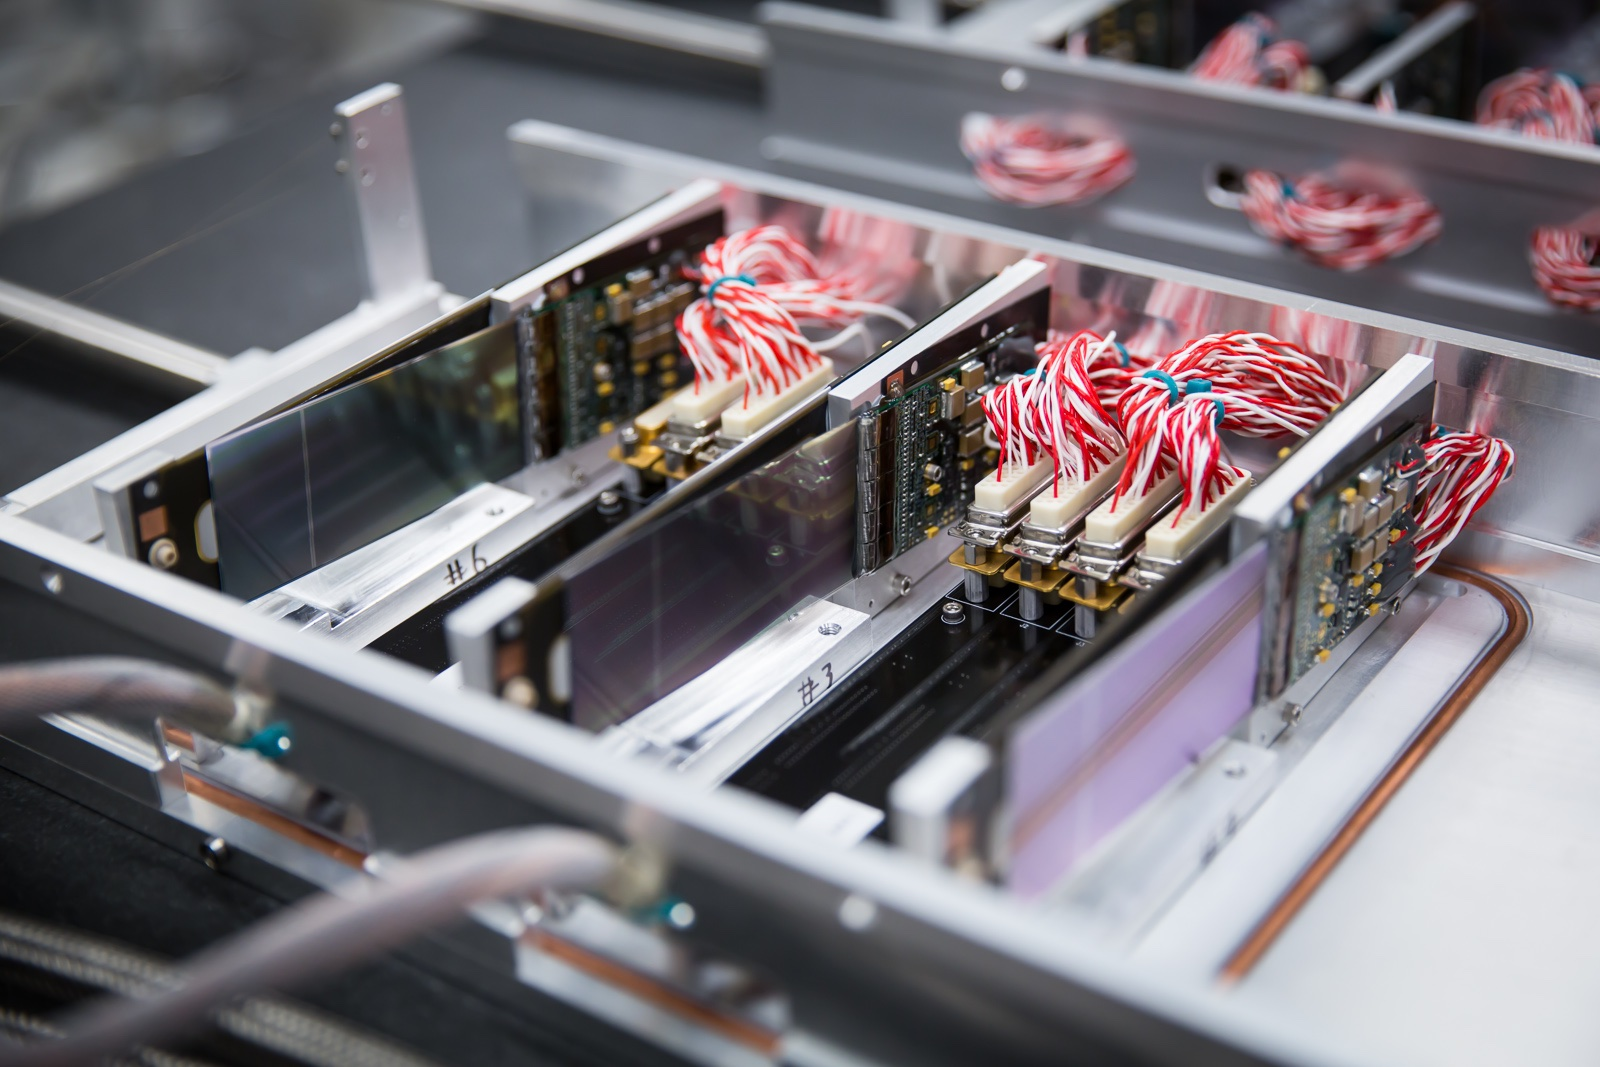
\includegraphics[width=\textwidth]{detector/figs/l123}
    \caption{One of two U-channels for L1--3, fully assembled.
    The beam direction is left to right; the scan wires and motion lever are visible on the left.}
    \label{fig:l123}
\end{figure}

\begin{figure}[htp]
    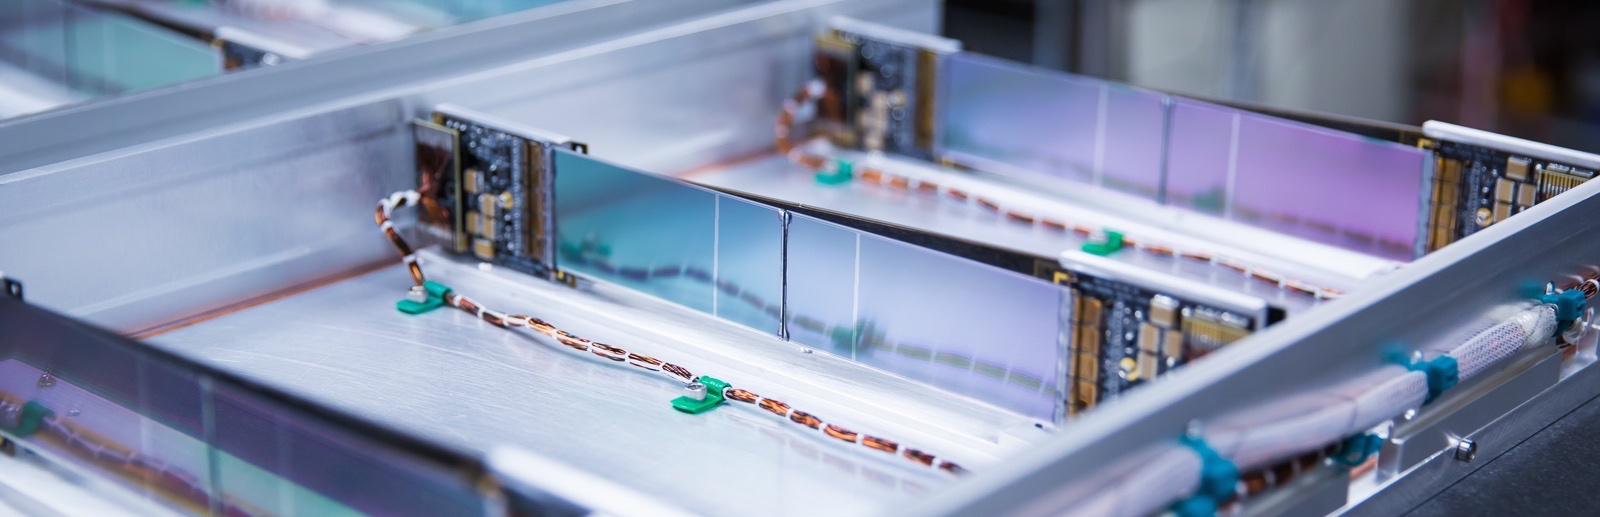
\includegraphics[width=\textwidth]{detector/figs/l456}
    \caption{One of two U-channels for L4--6, fully assembled.
    The beam direction is left to right.}
    \label{fig:l456}
\end{figure}

Each U-channel is supported at three points using kinematic mounts, which guarantee repeatable positioning when the U-channels are installed.
The L4--6 U-channels rest on three kinematic mounts.
The L1--3 U-channels rest on two kinematic mounts, which serve as a hinge at the downstream end of the U-channels, and are supported on the upstream end by motion levers which tilt the U-channels up and down.
In addition to modules, the L1--3 U-channels carry scan wires so that the beam position can be measured relative to the silicon.

\begin{figure}[htp]
    \begin{center}
    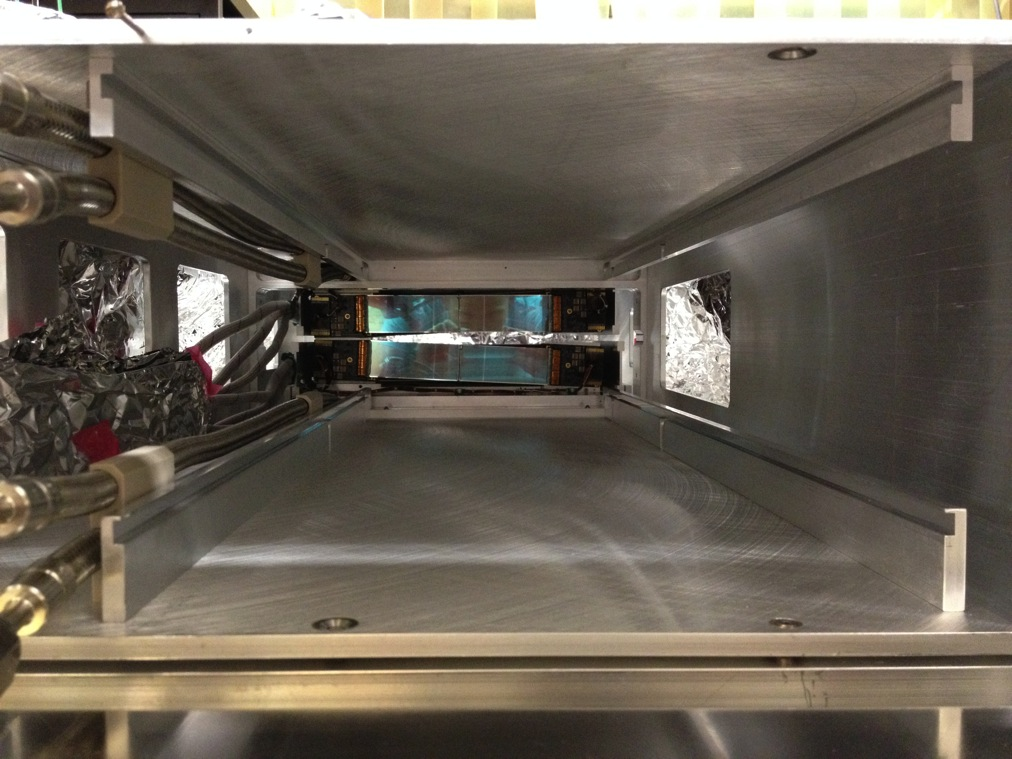
\includegraphics[width=0.8\textwidth]{detector/figs/drawers}
    \end{center}
    \caption{Inside the SVT box, looking downstream.
    The L4--6 U-channels are installed.
The rails for the L1--3 U-channels can be seen at the top and bottom. When the U-channels are installed, bearings on the U-channels roll along the horizontal slots until they drop down into the vertical slots, guiding the U-channel onto its kinematic mounts.
The cooling lines (in braided jackets) and cables (ends wrapped in foil) for the L4--6 U-channels are visible to the left.}
    \label{fig:drawers}
\end{figure}

\subsubsection{Survey}
\label{sec:svt_survey}

The SVT is surveyed to determine the positions of the sensors in the detector volume.
This serves two purposes.
First, surveying the SVT checks that it was assembled as designed, and allows adjustable components to be brought to their design positions.
Second, the precision of tracks reconstructed with the SVT is limited by the precision with which the sensor positions are known; the survey provides the initial knowledge of the detector geometry, which must be good enough to allow efficient track reconstruction, and close enough to the true geometry for track-based alignment (see Section \ref{sec:internal_alignment}) to work.

The basic tool for the SVT survey is a coordinate-measuring machine (CMM).
A CMM uses optical and/or touch probe measurements to locate target points in three dimensions.
%The silicon sensors were fabricated with fiducial markings that are easily measured optically.
%The bases of the pairing fixtures are a convenient reference frame for 
%The U-channels have conical fiducials meant for the module mounting surfaces and pins are simple shapes that can be located precisely with a touch probe, and the U-channels 

Because the SVT is assembled in a modular way, with repeatable positioning at each stage, the survey can be done in stages as well.
Each module is surveyed to find the positions of the silicon relative to the module mounting points.
Each U-channel is surveyed to find the positions of the module mounting points relative to the U-channel.
After the U-channels are installed in the SVT box, the SVT box is surveyed to find the positions of the U-channels relative to the SVT box; the U-channel kinematic mounts are adjusted during the survey to bring the U-channels to their nominal positions.
Finally, after the SVT box is installed in the pair spectrometer vacuum chamber, the SVT box is surveyed to find the position of the SVT box relative to the rest of the detector.

\subsection{Power and Data Acquisition}
\label{sec:power_daq}
The power and data paths for the SVT are constrained.
All signals must pass through a pair of 8-inch vacuum flanges at the upstream side of the analyzing magnet, so the number of signals has to be reduced.
The closest available rack for the SVT power supplies and DAQ is 20 meters from the alcove where HPS is installed, so the analog APV25 output signals have to be converted to digital optical signals.
Therefore HPS digitizes the signals and regulates the low-voltage power supplies inside the vacuum chamber, on frontend boards (FEBs) that are mounted on a cooling plate next to layers 1--3.

\begin{figure}[htp]
    %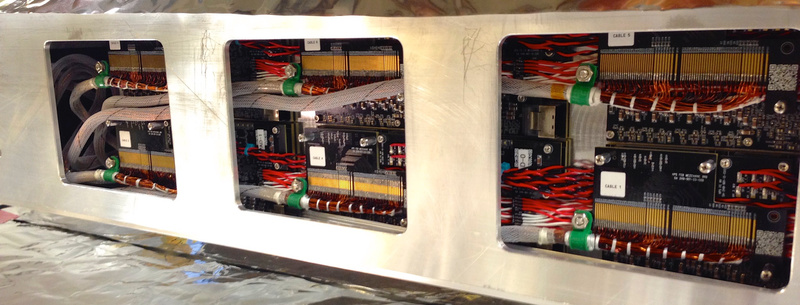
\includegraphics[width=\textwidth]{detector/figs/svt_febs}
    \begin{center}
    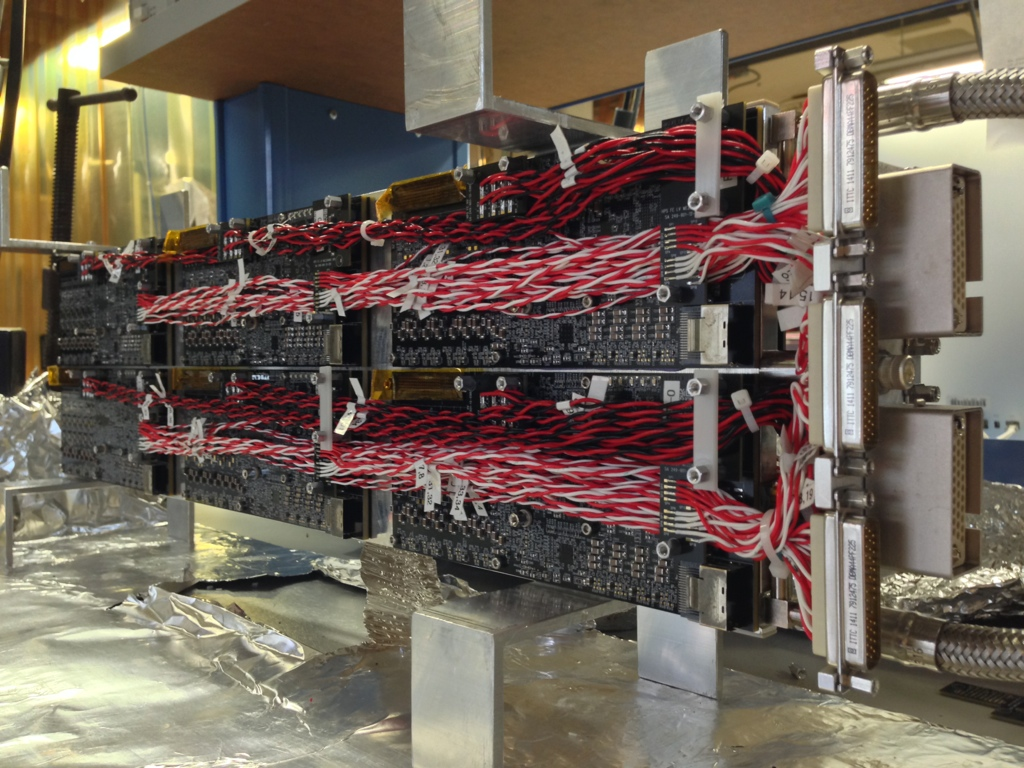
\includegraphics[width=0.8\textwidth]{detector/figs/febplate}
    \end{center}
    \caption{The SVT FEBs (frontend boards), mounted on their cooling plate. The red-and-white cables distribute low-voltage power to the FEBs; the red-and-black cables distribute high-voltage bias to the FEBs. The connectors for hybrid power, bias and data are covered with yellow Kapton tape. The mini-SAS connectors for high-speed data cables are at the bottom right of each FEB.}
    \label{fig:febplate}
\end{figure}

Each FEB can service four hybrids: a pair of L1--3 modules or a single L4--6 module.
A single bundle of impedance-controlled twisted pair magnet wire connects each FEB to its set of hybrids, carrying low-voltage power, high-voltage sensor bias, analog APV25 output signals, and digital control and trigger signals.

Each FEB digitizes the output signals from 20 APV25 chips.
Each differential current signal is converted to a voltage by a preamp and digitized by a 14-bit ADC.
Each FEB carries a single Xilinx Artix-7 FPGA, which packs the ADC data to be streamed off the FEB.
The FPGA also monitors the hybrid state and configuration.
All data and control signals are on a single high-speed data link, carried by a standard mini-SAS cable.

The FEBs also distribute low-voltage power to the hybrids.
A single voltage supplied to the FEB is split into four independent voltages (one per hybrid) using a combination of switching and linear voltage regulators.
This improves noise performance and reduces the number of voltages that must be passed into the vacuum chamber.
High-voltage sensor bias is also routed through the FEBs, but is passed through directly.

Two sets of cables connect the FEBs to the vacuum chamber flanges: mini-SAS cables carrying digital signals, and twisted pair cables carrying low-voltage power and high-voltage bias.
In both cases, the number of connections is too high for conventional vacuum feedthroughs.
Instead, HPS uses ``flange boards.''
Each board has a vacuum side and an air side, to which connections are made using solder or standard connectors.
The middle section of the board carries signal traces but is kept smooth; the board is then passed through a machined gap in the vacuum flange, and epoxy is poured to fill the space around the board: see Figure \ref{fig:flangeboard_test}.
The flange on beam-right carries two flange boards: one for low voltage and one for high voltage.
The flange on beam-left carries four signal flange boards (one of which is shown in Figure \ref{fig:flangeboard}), which use fiber transceivers on the air side to convert the electrical signals to optical signals.

\begin{figure}[htp]
    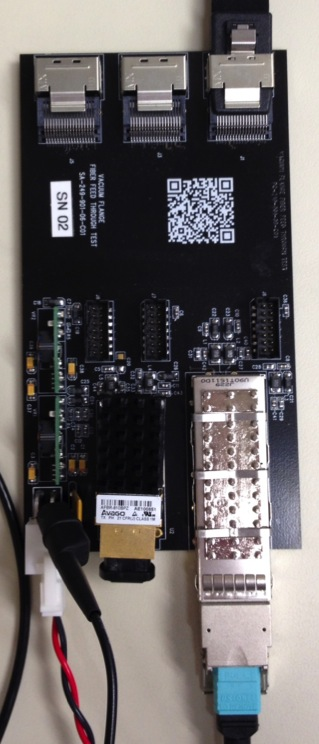
\includegraphics[angle=90,width=\textwidth]{detector/figs/flangeboard}
    \caption{One HPS signal flange board.
    The left side of the board operates in vacuum, and has three mini-SAS electrical connectors for high-speed data cables, which connect to the FEBs.
The right side of the board operates in air, and has two MPO multi-fiber connectors for data and control signals.}
    \label{fig:flangeboard}
\end{figure}

\begin{figure}[htp]
    \begin{center}
    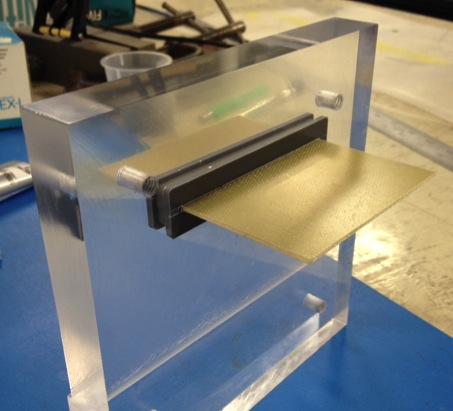
\includegraphics[width=0.7\textwidth]{detector/figs/flangeboard_test}
    \end{center}
    \caption{Test of the flange board potting process.}
    \label{fig:flangeboard_test}
\end{figure}

The low and high voltages for the SVT are supplied by Wiener MPOD power supplies.
The low-voltage supplies use sense lines to regulate the voltage actually supplied to the FEBs, and compensate for voltage drop in the cables.

The core of the SVT DAQ is the RCE platform.
This is a general-purpose DAQ system developed at SLAC.
The system is built on the ATCA (Advanced Telecommunications Computing Architecture) industry standard and is housed in a standard ATCA crate.

The data processing, trigger handling, and event building is done on a COB (Cluster On Board) blade, which carries a set of daughterboards: four DPMs (Data Processing Modules) and one DTM (Data Transport Module).
All of these are generic hardware that can be used for any experiment using the RCE platform.
The only HPS-specific hardware is the (RTM) Rear Transition Module, which interfaces the COB to the fiber bundles connected to the signal flange boards.
The SVT DAQ uses two fully loaded COBs and two RTMs.
Each DPM contains two data processing nodes, each of which runs a Xilinx Zynq system-on-a-chip which integrates an ARM processor (running the Linux operating system) and an FPGA.
The nodes can therefore process and reduce data on the FPGA at high speed, and perform high-level functions on the processor.
The DTM contains a single node, which handles timing and trigger distribution.
An implementation of the JLab TI (Trigger Interface) module is integrated in the DTM firmware for HPS.

On each trigger, the SVT DAQ reads out six 14-bit samples for every one of 23040 APV25 channels.
This is far too much data to store in full, so the DAQ applies a data reduction threshold to select the channels to be recorded in the event.
The threshold rule used in the 2015 run was for three samples to exceed the channel pedestal by at least three times the channel noise.
The channel pedestal and noise are taken from offline calibrations, and are the mean and standard deviation of samples from the channel in the absence of an input signal.

\begin{figure}[htp]
    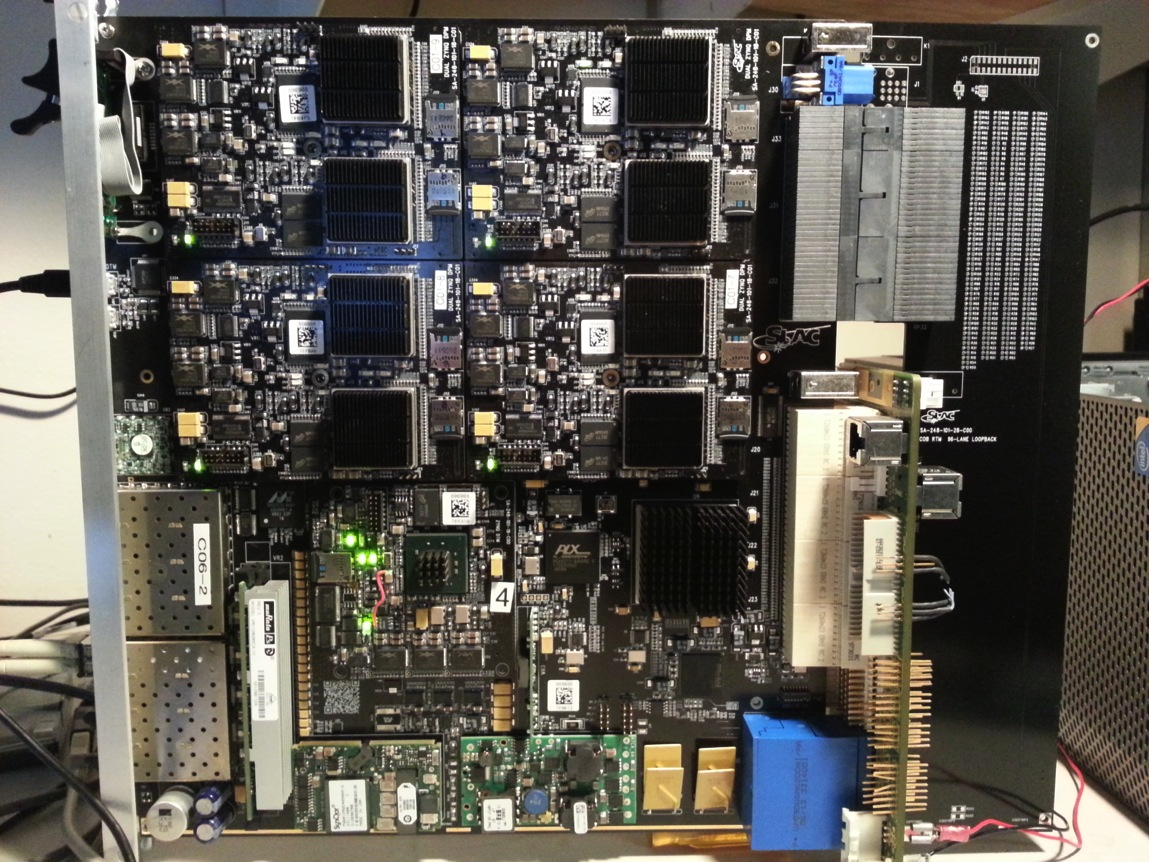
\includegraphics[width=\textwidth]{detector/figs/rce}
    \caption{The RCE system. The COB (Cluster On Board) blade on the left hosts four RCE (Reconfigurable Cluster Element) daughterboards, which perform the data processing. The RTM (Rear Transition Module) on the right interfaces with fibers carrying data from the flange boards. The COB and RTM would normally be housed in an ATCA crate.}
    \label{fig:rce}
\end{figure}

\subsection{Services}
\label{sec:svt_services}
All the services needed to operate the SVT --- motion, cooling, and power --- must be supplied from outside the vacuum.
These enter the vacuum through flanges on the upstream vacuum chamber.

Three linear shifts provide independent control of the upper and lower U-channels for layers 1--3, and the target frame.
Each linear shift is driven by a stepper motor; the three stepper motors are powered and controlled by a Newport XPS controller.
The motor turns a lead screw to create precise linear motion, which is transmitted inside the vacuum chamber through a bellows.

The SVT uses two independent cooling loops.
The silicon sensors need to be kept cold (below $0^\circ$ C) to prevent reverse annealing.
Reverse annealing is an effect where the performance of radiation-damaged silicon worsens after exposure to high temperatures.
The FEBs only need cooling to remove the heat they generate, and their cooling loop can run near room temperature.
%The SVT proper (sensors and hybrids, cooled through the U-channels) is kept near $-10^\circ$ C to prevent reverse annealing of the silicon.
%The FEBs (cooled through their cooling plate) are kept 

The SVT is cooled by circulating cooling fluid through copper lines that are pressed into the U-channels.
As discussed in Section \ref{sec:svt_mechanical}, the modules and half-modules are engineered to provide short and parallel cooling paths from the sensors and readout chips to the U-channels.
A low-viscosity fluid is required to keep flow rates high at low temperature; HPS uses Novec 7000, a hydrofluoroether compound.
The SVT chiller operates at a setpoint of $-20^\circ$ C.
The cooling flow is split between the top and bottom halves of the SVT before it enters the vacuum chamber through ceramic feedthroughs; the L1--3 and L4--6 U-channels are connected in series.

The FEBs are cooled by circulating distilled water through copper lines pressed into the FEB cooling plate.
The FEB components are kept in direct thermal contact with the cooling plate: the heat-generating components are on the side of the board that faces the cooling plate, and the plate has machined pockets lined with thermally conducting pads.
The FEB chiller operates at a setpoint of $25^\circ$ C.

Power provision to the SVT and FEBs is explained in Section \ref{sec:power_daq}.

\section{Electromagnetic Calorimeter and Trigger}
The HPS ECal is a homogeneous crystal calorimeter, containing 442 lead tungstate (PbWO$_4$) scintillating crystals.
The ECal is based on the CLAS Inner Calorimeter (IC); the crystals are reused from the CLAS IC, and the basic design of each crystal module is unchanged.
The mechanical and electronic design of the HPS ECal was led by the same IPN Orsay group that built the CLAS IC.

The crystals have a trapezoidal shape, 16 cm long, with front faces $1.3\times 1.3$ cm$^2$ and back faces $1.6\times 1.6$ cm$^2$.
Lead tungstate has a fast time response, which allows for good time resolution and high pileup tolerance.
An avalanche photodiode (APD) is glued to the back face of each crystal for readout.
Two LEDs (one red, one blue) are mounted on the front face of each crystal, and are used to monitor the stability of the readout gain and radiation damage to the crystals.

The ECal is split into top and bottom halves; each half contains 5 rows of 46 crystals, except for the innermost row which has 9 crystals removed to avoid the region of highest beam background (this gap in row 1 is known as the ``electron gap'').
The crystals are spaced as closely as possible.
Since the crystals are tapered, they fan out to the sides and an incident particle will typically not hit a crystal head-on.
Scintillator response is sensitive to the crystal temperature, so the ECal is surrounded by a thermal enclosure.
The innermost rows of crystals are 2 cm from the beam plane, and the front plane of the ECal is 139.3 cm from the nominal target position.

\begin{figure}[htp]
    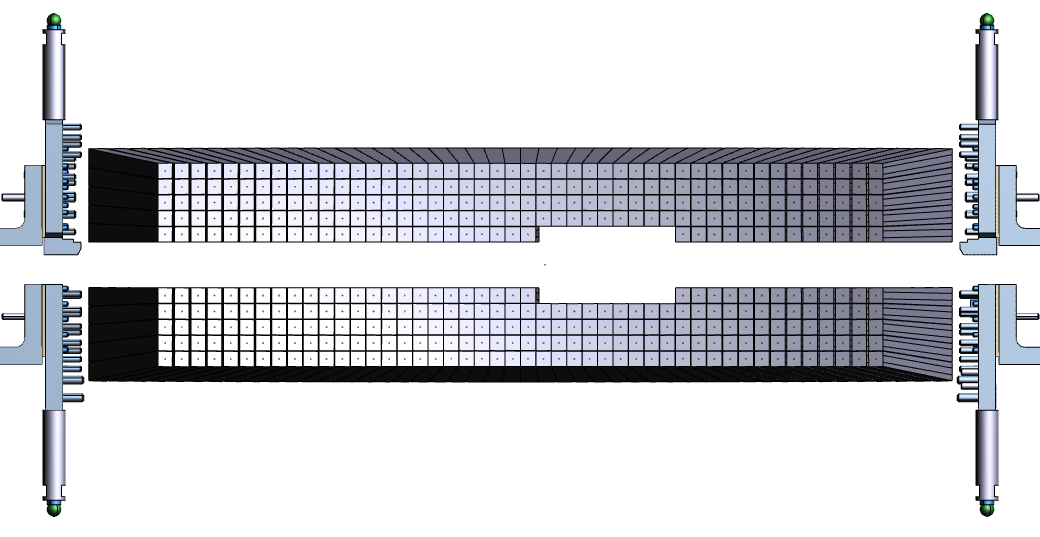
\includegraphics[width=\textwidth]{detector/figs/ECal}
    \caption{Beam's-eye-view of the ECal.
    18 crystals (the ``electron gap'') in the innermost rows are missing, to make space for the oval bulge in the ECal vacuum chamber (Figure \ref{fig:ecal_chamber}).
    The thermal enclosure that surrounds the ECal is not shown.}
    \label{fig:ecal}
\end{figure}

\begin{figure}[htp]
    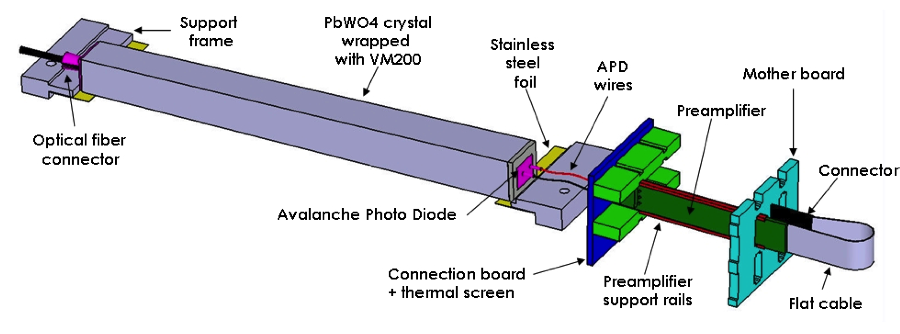
\includegraphics[width=\textwidth]{detector/figs/ecal_module}
    \caption{One ECal crystal with its readout electronics. The optical fiber was used in the CLAS IC for calibration and monitoring, but was removed for HPS. HPS uses LEDs mounted directly in front of the crystals.}
    \label{fig:ecal_module}
\end{figure}

\subsection{Readout and Trigger}
\label{sec:trigger}
Each ECal crystal has its own preamplifier.
The preamp output signals are routed through a motherboard and out to cables, which connect to FADC250 digitizer boards in VXS crates.

The FADC250 (FADC for short) is a general-purpose readout board developed at Jefferson Lab.
Each FADC board has 16 input channels, which are digitized continuously to 12-bit precision at 250 MHz.
The digitized samples are stored in pipelines so they can be read out in response to a trigger.
Several readout modes exist, and the FADC has the capability to perform pulse integration or emulate a constant-fraction TDC, but HPS uses the readout mode that outputs a window of 100 samples around the trigger time.
This allows pulse fitting, for the best possible time resolution.

The FADC is also the first step in the trigger chain; the trigger chain is implemented entirely using VXS boards developed by Jefferson Lab as a general-purpose trigger framework for experiments at the lab.
The digitized samples are passed to an algorithm that continuously looks for threshold crossings, and integrates the signal amplitude within a fixed window around each threshold crossing.
The integrated amplitude is then converted to an energy using calibrated values of pedestal and gain.
Hits found in this way (crystal position, energy, time of threshold crossing) are reported to the Global Trigger Processor (GTP) every 32 ns.

The two GTP boards (one per ECal half) cluster the hits according to a simplified algorithm.
According to this algorithm, a cluster is a set of hits in a $3\times 3$ block of crystals, where the center hit is at least 50 MeV and is a local maximum in energy, and the other hits in the cluster are within 16 ns of the center hit.
Both GTP boards report clusters (center crystal, center hit time, number of hits, total energy) to the single Subsystem Processor (SSP) board.

The Subsystem Processor (SSP) makes the trigger decision.
For the HPS physics trigger, the clusters from the two halves of the ECal are paired up, and each pair is tested against the defined trigger cuts.
If a pair meets the trigger requirements, a trigger is sent to the Trigger Supervisor board (TS), which then distributes the trigger to the Trigger Interface (TI) boards installed in all detector readout subsystems.
If any subsystem is not ready to accept a trigger, or if the trigger follows too closely after another trigger (as defined by rules configured in the TS), the TS will reject the trigger.

A total of six trigger types are defined in the SSP.
The HPS physics trigger is nicknamed ``pairs-1'' and is detailed in the next section.
A looser variant of the same trigger is nicknamed ``pairs-0'' and is used for diagnostics.
A single-cluster trigger tuned to trigger on electrons near the beam energy (elastic scatters) is called ``singles-1,'' and a looser variant is ``singles-0.''
To keep the rates of ``pairs-0,'' ``singles-1'' and ``singles-0'' triggers low as a fraction of the total trigger rate, they are prescaled so only one in $2^N$ ($N$ in the range of 10 to 13, depending on the trigger) of each trigger is accepted.
A pulser trigger generates a constant rate of triggers at 100 Hz regardless of detector conditions.
A ``calibration'' trigger is used for cosmic ray calibration of the ECal when the beam is off, triggering on a pair of scintillator paddles mounted under the ECal.

The total trigger rate during normal operations in the 2015 run was roughly 19 kHz, of which 16.6 kHz was pairs-1.

Measurements of livetime (the fraction of time during which the DAQ is sensitive to triggers) are important for normalizing the data.
Two measurements of livetime are available.
The first measurement uses the Faraday cup (see Section \ref{sec:beamline_hallb}) and a gating signal output by the trigger system which indicates whether the DAQ is live.
In addition to a scaler that records the Faraday cup measurement of integrated beam charge, a ``gated Faraday cup scaler'' records integrated beam charge with the DAQ live.
The gated Faraday cup scaler is the standard measurement of integrated charge used by CLAS.
The ratio of the gated to ungated scalers measures the fraction of the integrated beam charge which was accumulated with the DAQ live.
The second measurement uses the pulser trigger: the pulser trigger fires at a constant rate of 100 Hz, so the number of pulser triggers actually recorded is a direct measurement of the livetime.
Section \ref{sec:luminosity} discusses how these measurements compare, and why the pulser livetime is used for this analysis.

\subsection{Trigger Cuts}
\label{sec:trigger_cuts}

The HPS physics trigger is tuned to maximize efficiency for heavy photon decays: $e^+e^-$ coincidences with total energy near the beam energy.
For reasons explained below, there is no attempt to impose a minimum total energy requirement.
The main single-particle backgrounds are elastic scatters (electrons with energy near the beam energy) and bremsstrahlung photons.
The main two-particle background is wide-angle bremsstrahlung, where both the electron and photon hit the ECal.

A cluster reported to the SSP will not have energy equal to the incident particle, or even to the energy the full HPS reconstruction would compute for that cluster.
First, the FADCs are calibrated such that the reported energy of a hit equals the energy deposited in the crystal; whenever a particle showers in the ECal, some energy is absorbed in the vacuum flange in front of the ECal, penetrates through the back of the ECal, or escapes through the gaps between crystals.
These effects are compensated for in the full reconstruction but are ignored in the trigger.
Second, the GTP imposes a $3\times 3$ limit on the dimensions of a cluster, even though a single shower can deposit energy in a larger area.
For these reasons, the energy thresholds used in the trigger cuts are rather lower (by roughly a factor of 0.8) than would be expected based on true particle energies.

Furthermore, many particles hit the ECal in or near the innermost row of crystals.
For these particles, much of the shower is lost in the beam gap and the energy of the cluster can be much less than the particle energy.
Since these may still be desirable events (many decays from lower-mass heavy photons land in the innermost row of crystals), the trigger cuts mostly avoid imposing strong minimum requirements on cluster energy or total energy.

The time coincidence between the top and bottom clusters is required to be within 12 ns.
This allows for time walk; since the hit time reported by the FADC is a simple threshold crossing with a low threshold, time walk can be substantial.

The SSP applies an initial requirement on the energy and size of each cluster; it only considers clusters with energy between 54 and 630 MeV, and at least 1 hit.
For a pair, the sum of the cluster energies is required to be between 180 and 860 MeV, and the difference is required to be less than 540 MeV.
The minimum hit requirement is obviously trivial; the minimum cluster energy requirement is largely redundant with the GTP requirement on the center hit energy.
Of the other requirements, the most important is the maximum energy sum requirement: most of the events rejected by this cut are pairs of two beam-energy electrons.

The coplanarity cut is intended to select $e^+e^-$ events.
On average, $e^+e^-$ events should be symmetric around the beam axis (the line pointing along the beam direction at the target, starting at the beam spot).
Events with two electrons will usually have both clusters on beam-right, and will fail this cut.
The cut requires that the two clusters be on opposite sides of the beam axis: the azimuthal angle of each cluster is computed relative to the beam axis, and the difference between the two angles is required to be within $\pm 30^\circ$ of $180^\circ$.
(In practice, this cut is implemented as a mask of pairs of cluster positions that satisfy this cut.)

The energy-distance cut acts on the lower-energy cluster of the pair, and imposes the requirement $E_{low}+(5.5\text{ MeV/mm})r_{low}>600$ MeV, where $E_{low}$ is the cluster energy and $r_{low}$ is the cluster distance from the beam axis.
Restated as $E_{low}/(600\text{ MeV})+r_{low}/(600/5.5\text{ mm})>1$, the effect of this cut is to reject the pair if the lower-energy cluster is low-energy and close to the beam axis.
This primarily rejects wide-angle bremsstrahlung events, where the photon is typically the lower-energy particle, and is usually close to the beam axis.
The cut also rejects beam-energy electrons that hit close enough to the ECal edge that most of the energy is lost; these would pass the cluster energy cuts, but are closer to the beam axis than a genuine low-energy charged particle would be.

\begin{table}[htp]
    \begin{center}
        \caption{Trigger cuts for the ``pairs-1'' trigger.
        %$r$ and $\phi$ are defined relative to the photon line 
        }
        \begin{tabular}{lc}   
            \hline \hline
            Time difference & $|t_{top}-t_{bot}|\le12$ ns \\
            Cluster energy & $54<E<630$ MeV \\
            Cluster size & $N_{hits}\ge 1$ \\
            Energy sum & $180<E_{top}+E_{bot}<860$ MeV \\
            Energy difference & $|E_{top}-E_{bot}|<540$ MeV \\
            Coplanarity & $|\phi_{top}-\phi_{bot}-180^\circ|<30^\circ$ \\
            Energy-distance cut & $E_{low}+(5.5\text{ MeV/mm})r_{low}>600$ MeV \\
            \hline \hline
        \end{tabular}
        \label{tab:trigger_cuts} 
    \end{center}
\end{table}

